\documentclass[conference]{IEEEtran}

\usepackage[T1]{fontenc}
\usepackage[utf8]{inputenc}
\usepackage{cite}
\usepackage{amsmath}
\usepackage{amssymb}
\usepackage{graphicx}
\usepackage{booktabs}
\usepackage{array}
\usepackage{tabularx}
\usepackage{multirow}
\usepackage{float}
\usepackage[caption=false,font=footnotesize]{subfig}
\usepackage{url}
\usepackage{newtxtext,newtxmath}
\usepackage{microtype}
\usepackage[section]{placeins}
\usepackage[hidelinks]{hyperref}
\graphicspath{{main_updated_with_best_score/}}

\newcolumntype{Y}{>{\raggedright\arraybackslash}X}
\let\monocode\texttt
\renewcommand{\texttt}[1]{\textnormal{#1}}
\setlength{\emergencystretch}{2em}
\allowdisplaybreaks

\title{Leakage-Aware Preprocessing and Multi-Model Validation for the Spaceship Titanic Classification Task}

\author{
\IEEEauthorblockN{
Wang Han 2430034066 \quad Shen Yijie 2430034056 \quad Yang Yusong 2430034087\\
Jiang Zhibo 2430034031 \quad He Yuxiang 2230024062
}
\IEEEauthorblockA{group3}
}

\begin{document}

\maketitle

\begin{abstract}
This paper studies the Kaggle Spaceship Titanic binary classification task using a leakage-aware tabular machine-learning workflow. The proposed pipeline combines deterministic cleaning rules, train-only preprocessing statistics, engineered demographic and spending features, and branch-specific representations for Logistic Regression, Random Forest, XGBoost, LightGBM, and CatBoost. Under a stratified 80/20 local holdout protocol, LightGBM records the highest local validation accuracy (0.8171), while CatBoost records the strongest ROC-AUC (0.9125). For external submission feedback, the final XGBoost submission reaches a Kaggle public leaderboard score of 0.81412. These results suggest that careful preprocessing and representation design contribute as much to final performance as lightweight hyperparameter tuning in this tabular setting.
\end{abstract}

\begin{IEEEkeywords}
Spaceship Titanic, tabular machine learning, feature engineering, logistic regression, random forest, XGBoost, LightGBM, CatBoost
\end{IEEEkeywords}

\section{Introduction}
The Spaceship Titanic competition is a binary classification task in which the goal is to predict whether a passenger was transported to an alternate dimension based on demographic, cabin, travel-destination, and spending information~\cite{kaggle_spaceship_titanic}. As a representative tabular classification problem, it sits in a regime where strong tree-based methods, careful feature representation, and disciplined preprocessing often remain highly competitive relative to heavier deep tabular pipelines~\cite{borisov2024tabularsurvey,grinsztajn2022trees,mcelfresh2023nnsvstrees,grinsztajn2024betterdefault,tschalzev2024datacentric}. The study is organized around two layers:
\begin{itemize}
\item a minimal runtime layer for preprocessing, full training, and inference, and
\item an independent local validation layer for controlled model comparison, report-ready figures, and lightweight tuning.
\end{itemize}

The aim of this report is to document these components precisely: the preprocessing rules are written down explicitly, the model structures are formalized with equations and diagrams, and the parameter settings are reported in exact table form. This emphasis on explicit split handling, reproducible preprocessing, and transparent evaluation follows recent recommendations on leakage-aware machine-learning reporting~\cite{kapoor2023leakage,kapoor2024reforms}.

\section{Task and Dataset}
\subsection{Prediction Task}
Let $x_i$ denote the feature vector for passenger $i$ and let $y_i \in \{0,1\}$ denote the label, where $y_i=1$ corresponds to \texttt{Transported=True}. The task is to learn a mapping
\begin{equation}
\hat{y}_i = f(x_i)
\end{equation}
or, more generally, a probabilistic score
\begin{equation}
\hat{p}_i = P(y_i = 1 \mid x_i),
\end{equation}
which can later be converted to a binary decision with a threshold $\tau$:
\begin{equation}
\hat{y}_i =
\begin{cases}
1, & \hat{p}_i \ge \tau,\\
0, & \hat{p}_i < \tau.
\end{cases}
\end{equation}

\subsection{Dataset Summary}
This study uses the official Kaggle \textit{Spaceship Titanic} splits~\cite{kaggle_spaceship_titanic}:
\begin{itemize}
\item \texttt{train.csv}: 8693 labeled rows,
\item \texttt{test.csv}: 4277 unlabeled rows.
\end{itemize}

The raw training file contains the following columns:
\texttt{PassengerId}, \texttt{HomePlanet}, \texttt{CryoSleep}, \texttt{Cabin}, \texttt{Destination}, \texttt{Age}, \texttt{VIP}, \texttt{RoomService}, \texttt{FoodCourt}, \texttt{ShoppingMall}, \texttt{Spa}, \texttt{VRDeck}, \texttt{Name}, and the binary target \texttt{Transported}.

\begin{table}[H]
\caption{Dataset summary}
\label{tab:dataset_summary}
\centering
\begin{tabular}{lcc}
\toprule
Item & Value & Notes \\
\midrule
Training rows & 8693 & labeled \\
Test rows & 4277 & unlabeled Kaggle split \\
Positive-class ratio & 0.5036 & train only \\
Raw training missing values & 2324 & before cleaning \\
Raw test missing values & 1117 & before cleaning \\
Target column & \texttt{Transported} & binary label \\
\bottomrule
\end{tabular}
\end{table}

\begin{figure*}[!t]
\centering

\begin{minipage}[t]{0.42\textwidth}
\centering
\subfloat[Raw missing-value counts across train and test files.]{
    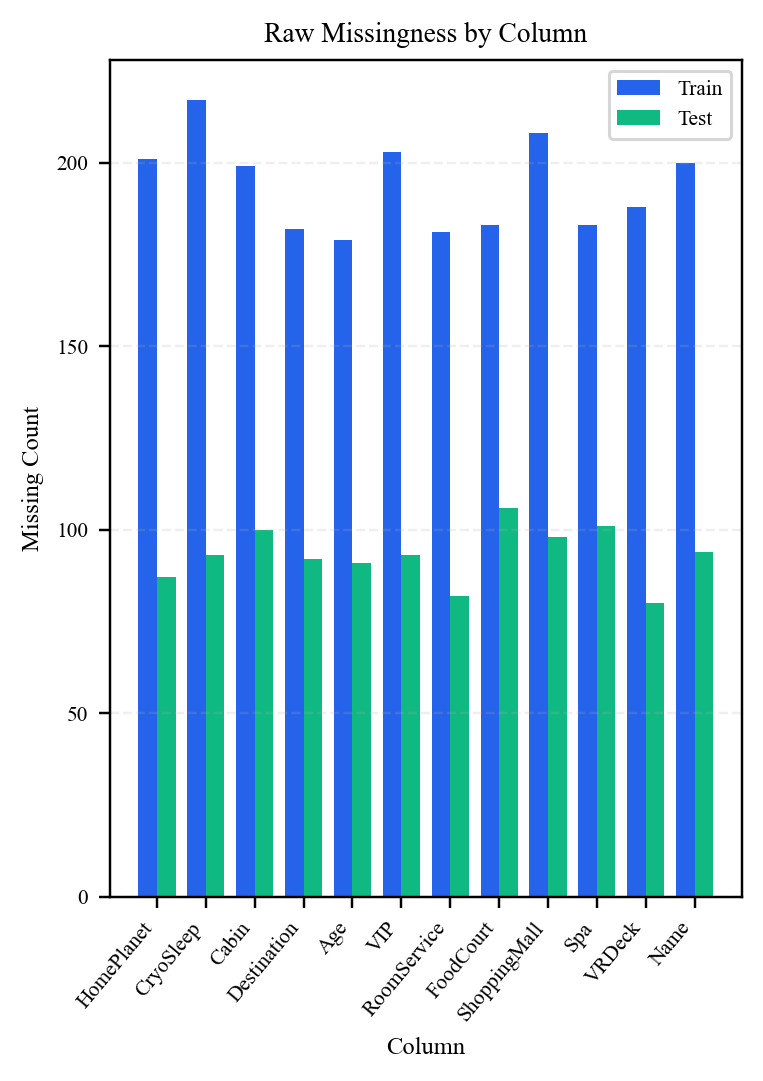
\includegraphics[width=\linewidth]{figures/raw_missingness_train_test.png}
    \label{fig:raw_missingness}
}
\end{minipage}
\hfill
\begin{minipage}[t]{0.53\textwidth}
\centering
\subfloat[Observed raw age distribution in the training data.]{
    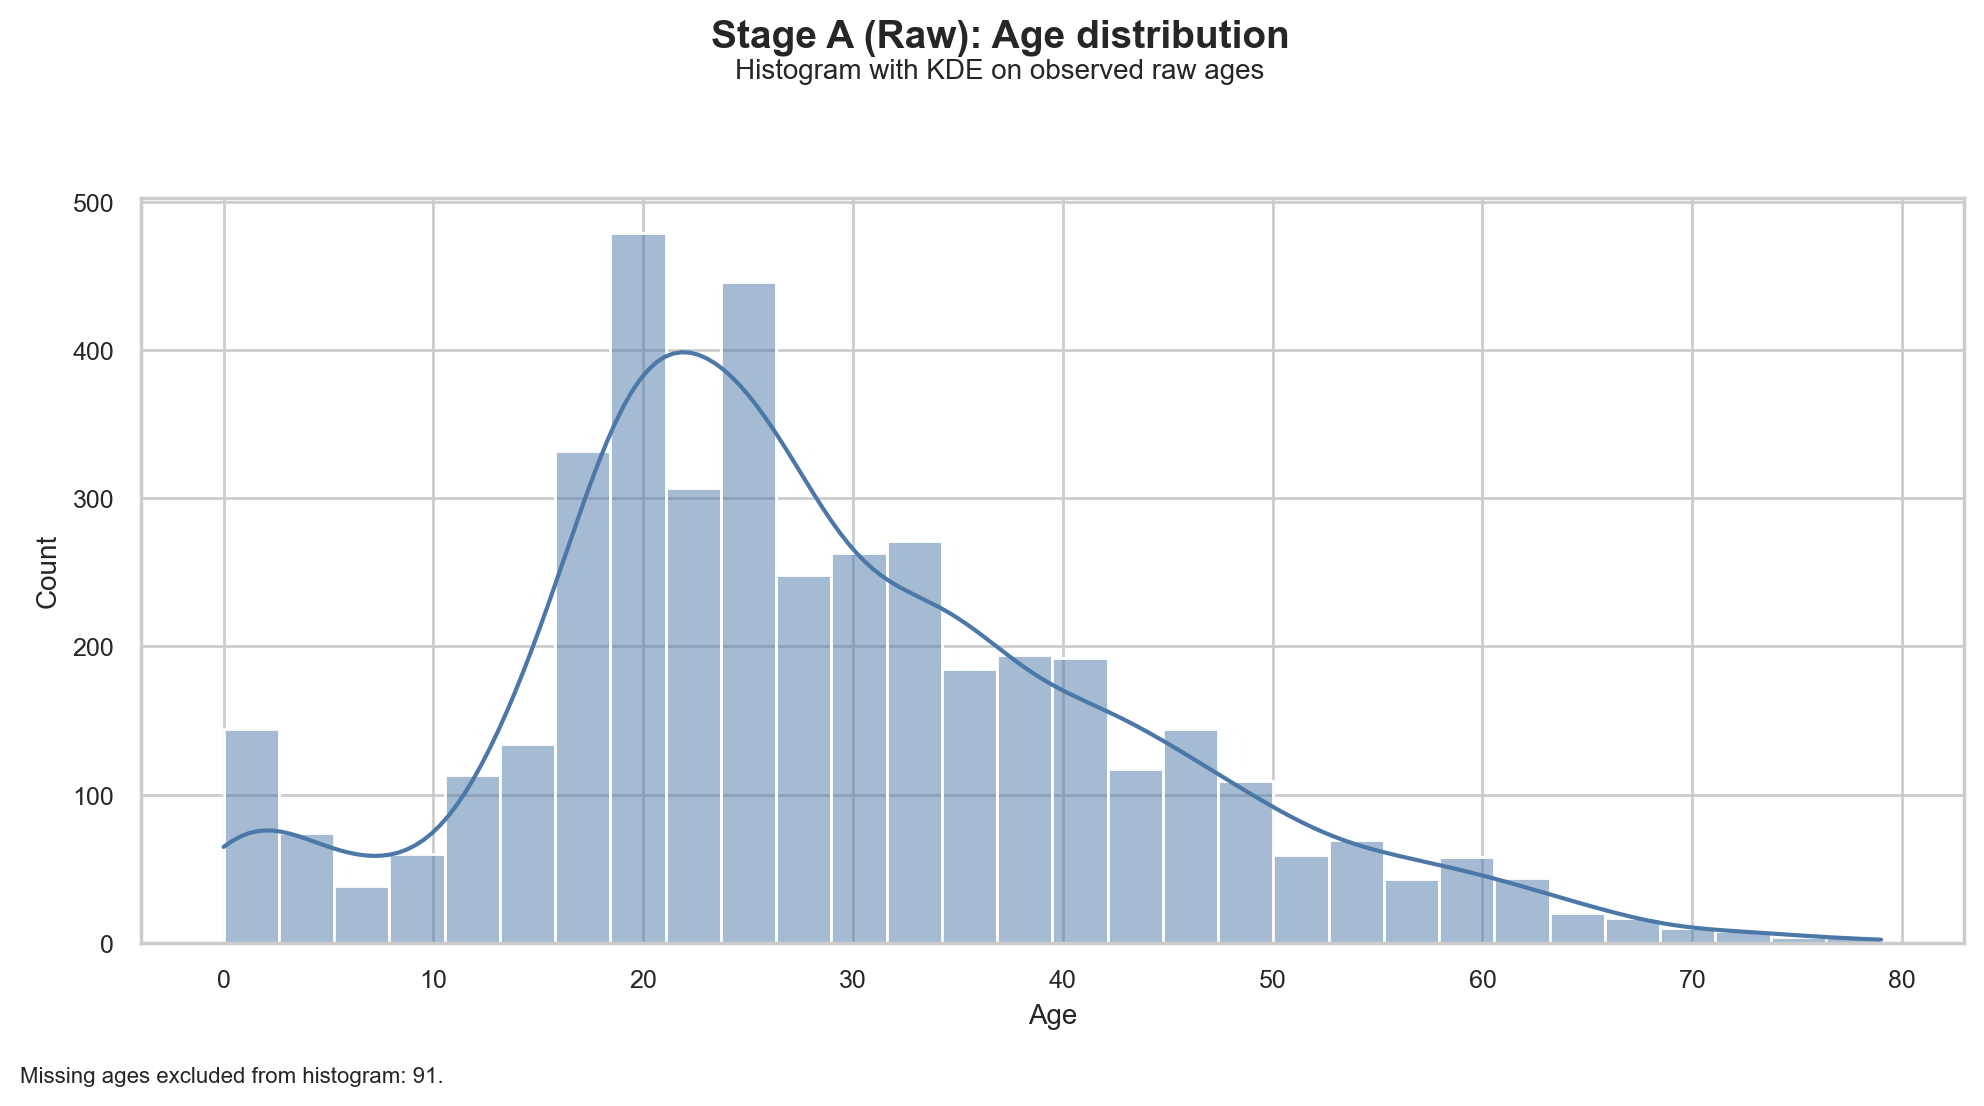
\includegraphics[width=\linewidth]{figures/eda/eda_age_distribution.png}
    \label{fig:eda_age_distribution}
}

\vspace{0.6em}

\subfloat[Raw HomePlanet distribution with missing values retained as a separate category.]{
    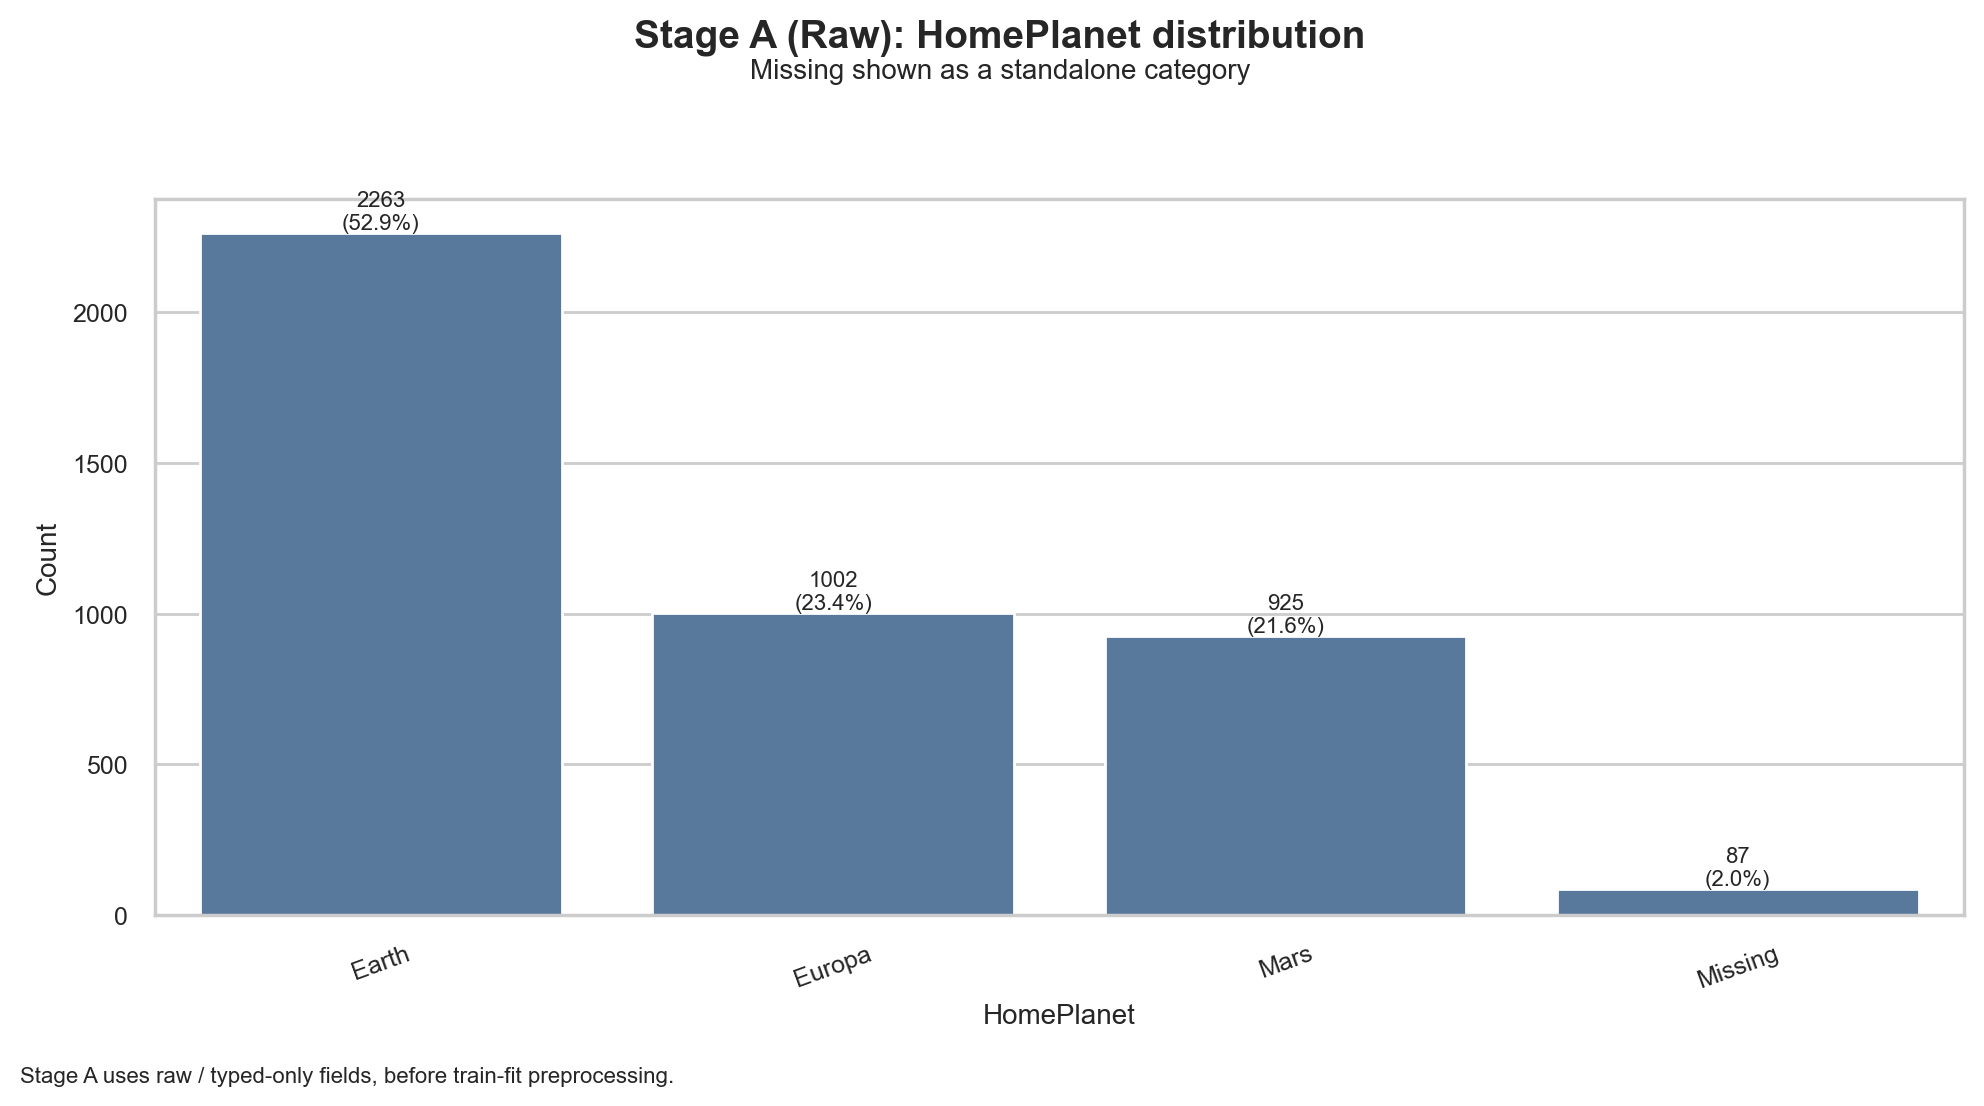
\includegraphics[width=\linewidth]{figures/eda/eda_homeplanet_distribution.png}
    \label{fig:eda_homeplanet_distribution}
}
\end{minipage}

\caption{Initial exploratory data analysis for the raw Spaceship Titanic dataset. The missingness plot compares raw train and test missing-value counts, while the age and HomePlanet plots summarize key demographic distributions before preprocessing.}
\label{fig:raw_eda_overview}
\end{figure*}

\section{Shared Preprocessing Pipeline}
\subsection{Overview}
The shared preprocessing logic is implemented in \texttt{preprocess.py}. Its purpose is to transform raw Kaggle records into a stable common feature frame and then branch that frame into model-specific representations. The pipeline first normalizes raw fields, then computes train-fit statistics, then creates shared engineered variables, and finally emits branch-specific bundles for each model family. This design treats cleaning and feature engineering as first-class parts of tabular model development rather than as a disposable preamble~\cite{chicco2022tips,tschalzev2024datacentric}.

\subsection{Raw Cleaning and Type Normalization}
The first stage applies two deterministic operations:
\begin{enumerate}
\item \textbf{Basic cleaning}: whitespace-only strings are converted to missing values and string fields are stripped of surrounding spaces.
\item \textbf{Type enforcement}: numeric columns such as \texttt{Age} and the five spending variables are coerced to numeric values; \texttt{CryoSleep} and \texttt{VIP} are normalized into string-valued boolean-like tokens (\texttt{True}/\texttt{False}); \texttt{Transported} is cast to integer 0/1.
\end{enumerate}
These operations follow standard recommendations for robust data cleaning and schema normalization before downstream modeling~\cite{chicco2022tips}.

\subsection{Identifier Parsing}
Two important structural columns are extracted directly from the raw identifiers:
\begin{align}
\texttt{PassengerId} &= \texttt{GroupID}\_\texttt{GroupMemberNo},\\
\texttt{Cabin} &= \texttt{Deck}/\texttt{CabinNum}/\texttt{Side}.
\end{align}

Concretely:
\begin{itemize}
\item \texttt{GroupID} is the substring before the underscore in \texttt{PassengerId}.
\item \texttt{GroupMemberNo} is the numeric suffix after the underscore.
\item \texttt{Deck}, \texttt{CabinNum}, and \texttt{Side} are obtained by splitting \texttt{Cabin} on the slash delimiter.
\item \texttt{Surname} is extracted as the last token in \texttt{Name}.
\end{itemize}

\subsection{Group-based Deterministic Rules}
The preprocessing stage also applies rule-based filling before statistical imputation:
\begin{itemize}
\item \texttt{HomePlanet}, \texttt{Destination}, and \texttt{VIP} can be filled from \texttt{GroupID} when all observed values inside the group are consistent.
\item Missing \texttt{CryoSleep} is inferred as \texttt{False} when any spend column is strictly positive.
\item Missing \texttt{CryoSleep} is inferred as \texttt{True} when the passenger is an adult, all five spend columns are observed, and total spend equals zero.
\item For rows with \texttt{CryoSleep=True}, all spend columns are deterministically forced to zero.
\end{itemize}
Such rules intentionally exploit structured consistency in the raw table before broader imputation, while keeping the logic explicit enough to audit during validation and later error analysis~\cite{josse2024missingconsistency,zhou2024missingreview}.

\begin{figure}[t]
\centering
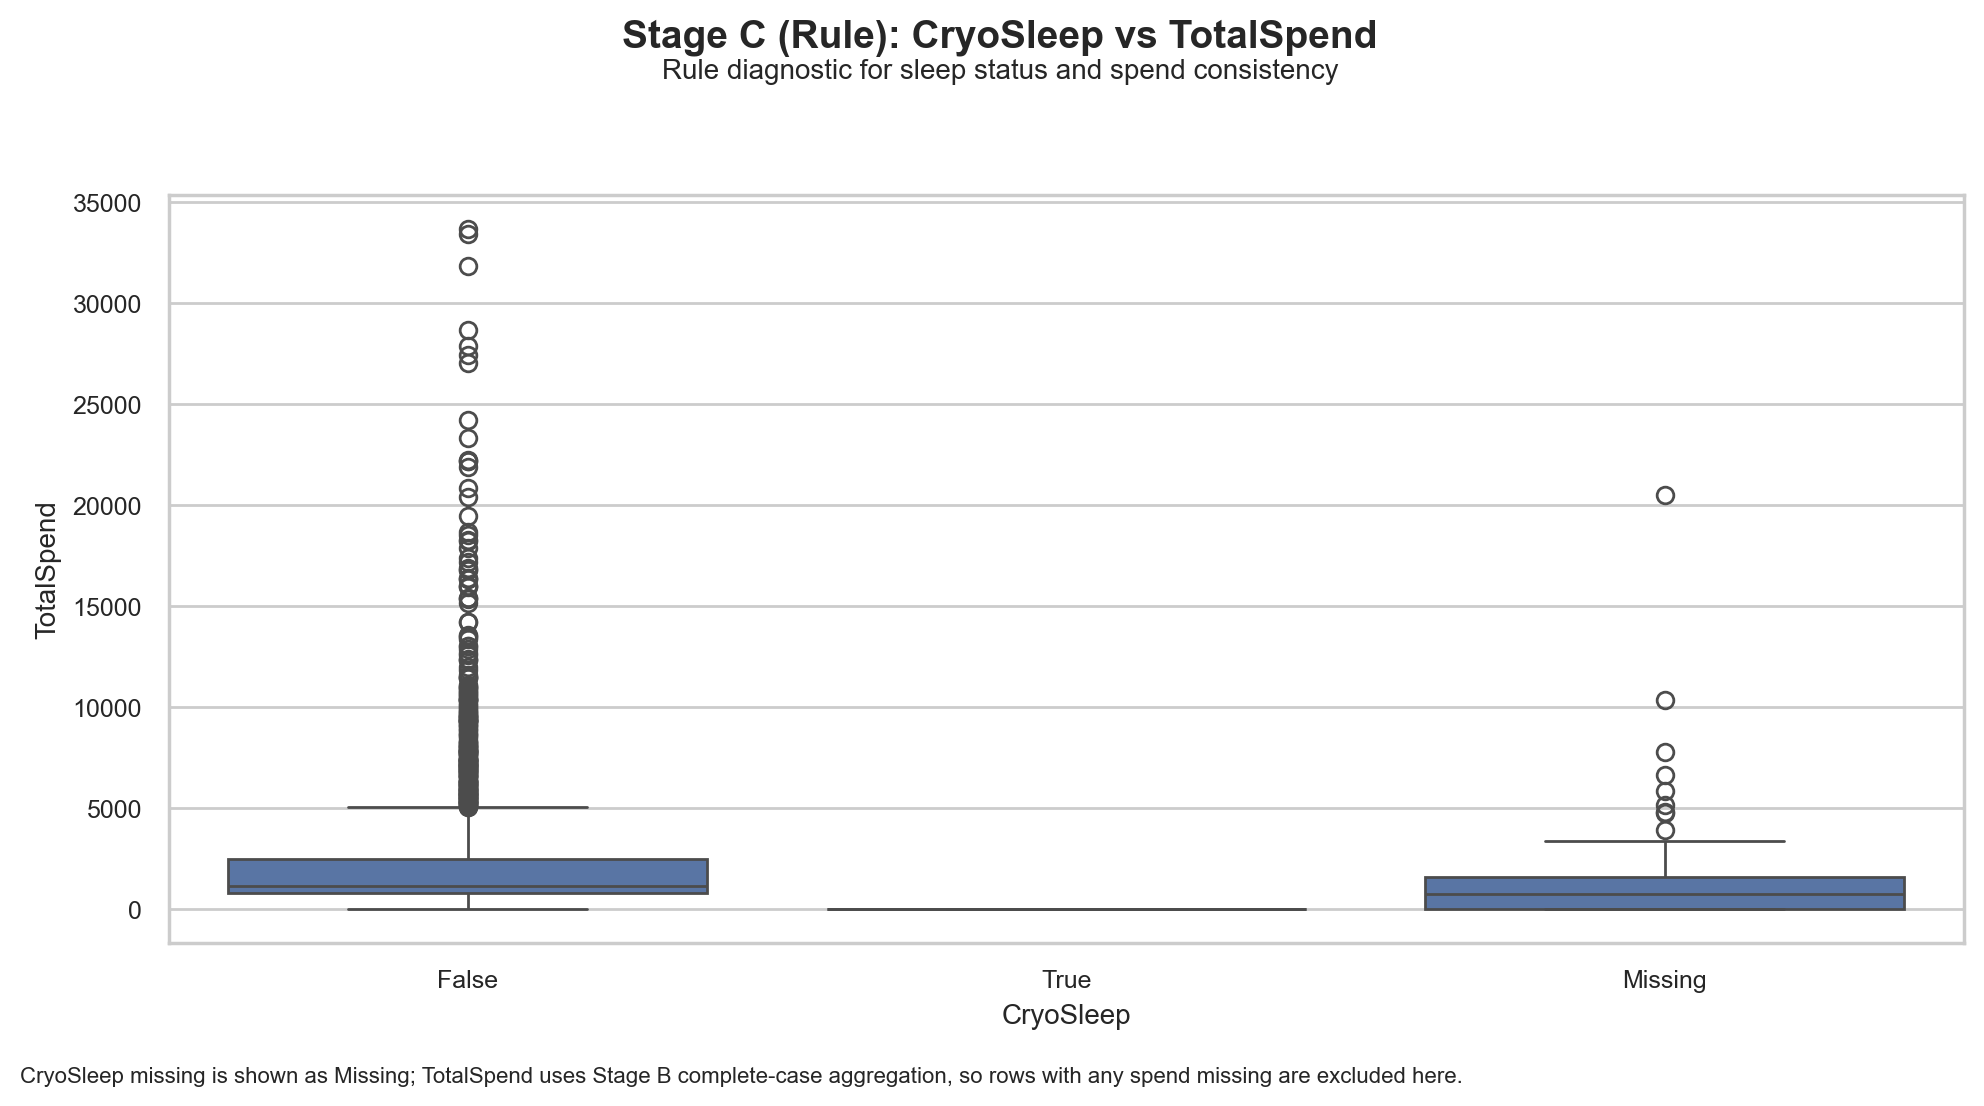
\includegraphics[width=\linewidth]{figures/eda/eda_cryosleep_totalspend_boxplot.png}
\caption{Relationship between CryoSleep status and TotalSpend, supporting the zero-spend consistency rule used during preprocessing.}
\label{fig:eda_cryosleep_totalspend}
\end{figure}

\subsection{Train-fit Statistics}
The pipeline explicitly separates train-fit statistics from later transformations, because reusing full-split statistics during validation would introduce leakage and weaken reproducibility claims~\cite{kapoor2023leakage,kapoor2024reforms}. The following quantities are fit on training data only:
\begin{itemize}
\item age median after out-of-range filtering,
\item \texttt{SurnameFreq} lookup map,
\item global spend medians,
\item positive-spend medians,
\item hierarchical spend medians,
\item \texttt{CabinNumBin} quantile edges.
\end{itemize}

Age normalization is defined as
\begin{equation}
\tilde{a}_i =
\begin{cases}
a_i, & 0 \le a_i \le 100,\\
\texttt{NaN}, & \text{otherwise},
\end{cases}
\end{equation}
and an indicator
\begin{equation}
\texttt{AgeWasOutOfRange}_i = \mathbb{1}[a_i < 0 \; \lor \; a_i > 100]
\end{equation}
is retained as a feature.

For spending variables, the imputation hierarchy is:
\begin{equation}
x_{ij}^{\text{filled}} =
\begin{cases}
0, & \texttt{CryoSleep}_i=\texttt{True},\\
\text{group median}, & \text{if a matching hierarchy bucket exists},\\
\text{positive median}_j, & \text{if other spend categories indicate positive spending},\\
\text{global median}_j, & \text{otherwise}.
\end{cases}
\end{equation}

The hierarchy buckets used for group medians are:
\begin{itemize}
\item \texttt{HomePlanet|Destination|VIP|Deck},
\item \texttt{HomePlanet|Destination|Deck},
\item \texttt{HomePlanet|Deck}.
\end{itemize}
This hierarchy favors transparent, split-local heuristics over heavier iterative imputers; stronger alternatives such as automatic model-selection-based imputation remain possible future upgrades rather than hidden preprocessing shortcuts~\cite{jarrett2022hyperimpute,josse2024missingconsistency,zhou2024missingreview}.

\begin{table}[t]
\caption{Train-fit statistics and deterministic rules}
\label{tab:train_fit_rules}
\centering
\begin{tabularx}{\linewidth}{l Y}
\toprule
Component & Implementation detail \\
\midrule
Age normalization & Values outside $[0,100]$ are flagged and treated as missing before median fill. \\
Surname frequency & \texttt{SurnameFreq} is computed from training surnames only; unseen test surnames map to 0. \\
Cabin binning & \texttt{CabinNum} is binned with train-fit quantile edges; missing values go to \texttt{CabinBin\_Missing}. \\
Spend imputation & Group median $\rightarrow$ positive median $\rightarrow$ global median, after enforcing the CryoSleep zero-spend rule. \\
Group size & Full preprocessing uses combined train+test passenger groups; local validation recomputes group size split-locally. \\
\bottomrule
\end{tabularx}
\end{table}

\subsection{Shared Engineered Features}
The project creates a large engineered feature set rather than relying on raw variables alone. Several of the most important features are defined explicitly below. This choice is consistent with recent evidence that feature design and data representation remain major determinants of tabular-model quality even when strong model families are already available~\cite{chicco2022tips,tschalzev2024datacentric,grinsztajn2024betterdefault}.

\subsubsection{Spend Features}
Let the spend columns be
\[
\begin{aligned}
\mathcal{S} = \{&\texttt{RoomService}, \texttt{FoodCourt}, \texttt{ShoppingMall},\\
                &\texttt{Spa}, \texttt{VRDeck}\}.
\end{aligned}
\]
Then
\begin{align}
\texttt{TotalSpend}_i &= \sum_{s \in \mathcal{S}} s_i,\\
\texttt{SpendCount}_i &= \sum_{s \in \mathcal{S}} \mathbb{1}[s_i > 0],\\
\texttt{IsZeroSpend}_i &= \mathbb{1}[\texttt{TotalSpend}_i = 0].
\end{align}

Luxury/basic decompositions are defined as
\begin{align}
\texttt{LuxurySpend}_i &= \texttt{Spa}_i + \texttt{VRDeck}_i,\\
\texttt{BasicSpend}_i
    &= \texttt{RoomService}_i + \texttt{FoodCourt}_i \notag\\
    &\quad + \texttt{ShoppingMall}_i,\\
\texttt{LuxuryShare}_i &= \frac{\texttt{LuxurySpend}_i}{\texttt{TotalSpend}_i + 1},\\
\texttt{SpendPerActiveCategory}_i &= \frac{\texttt{TotalSpend}_i}{\max(\texttt{SpendCount}_i, 1)}.
\end{align}

\begin{figure}[t]
\centering
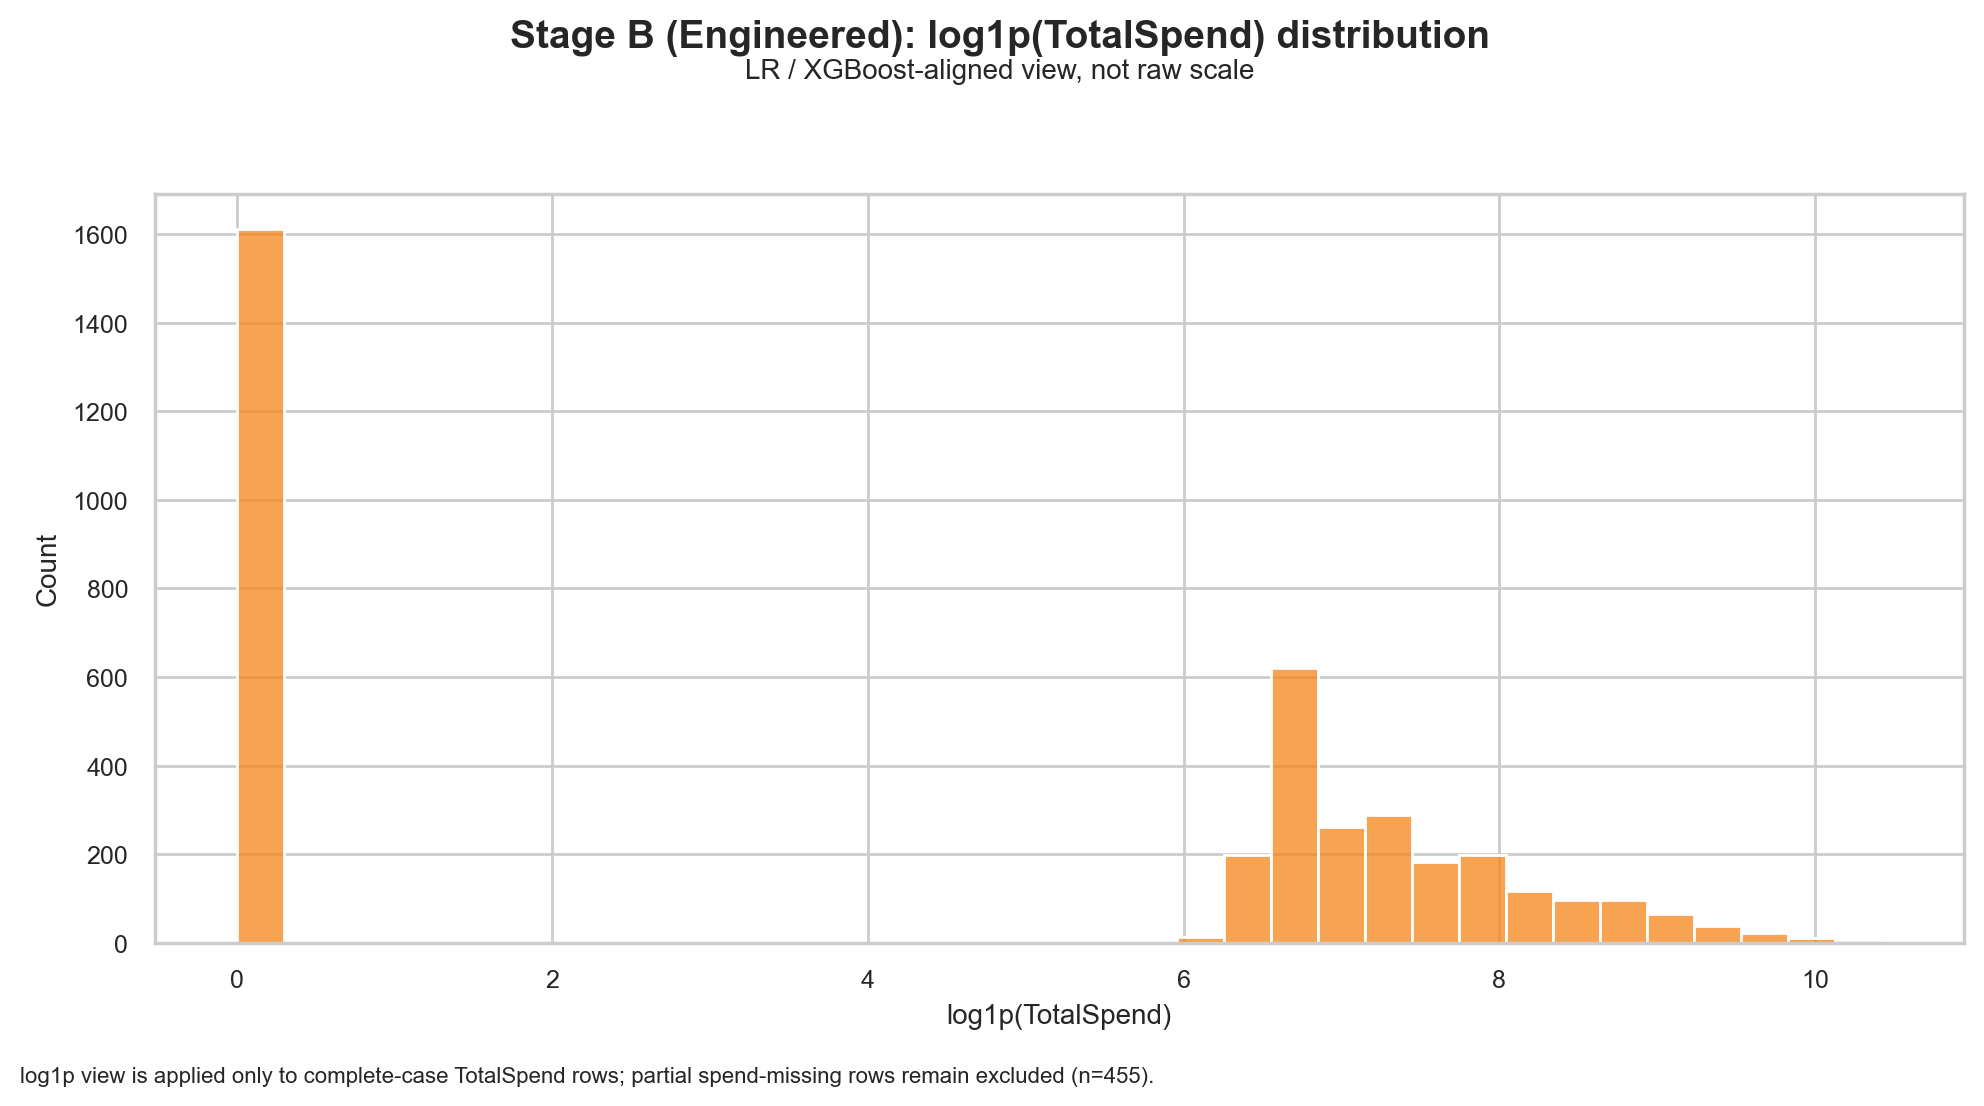
\includegraphics[width=\linewidth]{figures/eda/eda_totalspend_log1p_distribution.png}
\caption{Distribution of log-transformed TotalSpend used to reduce the skewness of spending-related features.}
\label{fig:eda_totalspend_log1p}
\end{figure}

\subsubsection{Age and Group Features}
Age segmentation is encoded through
\begin{align}
\texttt{IsChild}_i &= \mathbb{1}[\texttt{Age}_i < 18],\\
\texttt{IsSenior}_i &= \mathbb{1}[\texttt{Age}_i \ge 60],
\end{align}
and \texttt{AgeGroup} is binned into the semantic intervals:
\texttt{Child}, \texttt{Teen}, \texttt{YoungAdult}, \texttt{Adult}, \texttt{MiddleAge}, \texttt{Senior}, and \texttt{Unknown}.

Group features include
\begin{align}
\texttt{IsSolo}_i &= \mathbb{1}[\texttt{GroupSize}_i = 1],\\
\texttt{IsMultiPassengerGroup}_i &= \mathbb{1}[\texttt{GroupSize}_i > 1],\\
\texttt{GroupMemberIsLeader}_i &= \mathbb{1}[\texttt{GroupMemberNo}_i = 1].
\end{align}

\subsubsection{CatBoost-specific Extra Features}
For the CatBoost branch, extra features are added beyond the common base features:
\begin{align}
\texttt{GroupMemberRatio}_i &= \frac{\texttt{GroupMemberNo}_i}{\max(\texttt{GroupSize}_i,1)},\\
\texttt{CabinNumLog1p}_i &= \log(1+\max(\texttt{CabinNum}_i, 0)),\\
\texttt{SpendNonZeroRatio}_i &= \frac{\texttt{SpendCount}_i}{5},\\
\texttt{LuxuryToBasicRatio}_i &= \frac{\texttt{LuxurySpend}_i}{\texttt{BasicSpend}_i + 1},\\
\texttt{SpendPerGroupMember}_i &= \frac{\texttt{TotalSpend}_i}{\max(\texttt{GroupSize}_i,1)}.
\end{align}

Additional categorical interaction features are
\texttt{DeckCabinBin}, \texttt{DeckDestination}, and \texttt{SurnameFreqBin}.
Retaining and combining categorical signals in this way is consistent with recent findings on encoder choice and interpretable learning over large categorical domains~\cite{matteucci2023encoders,avanzi2023highcardinality}.

\begin{figure}[t]
\centering
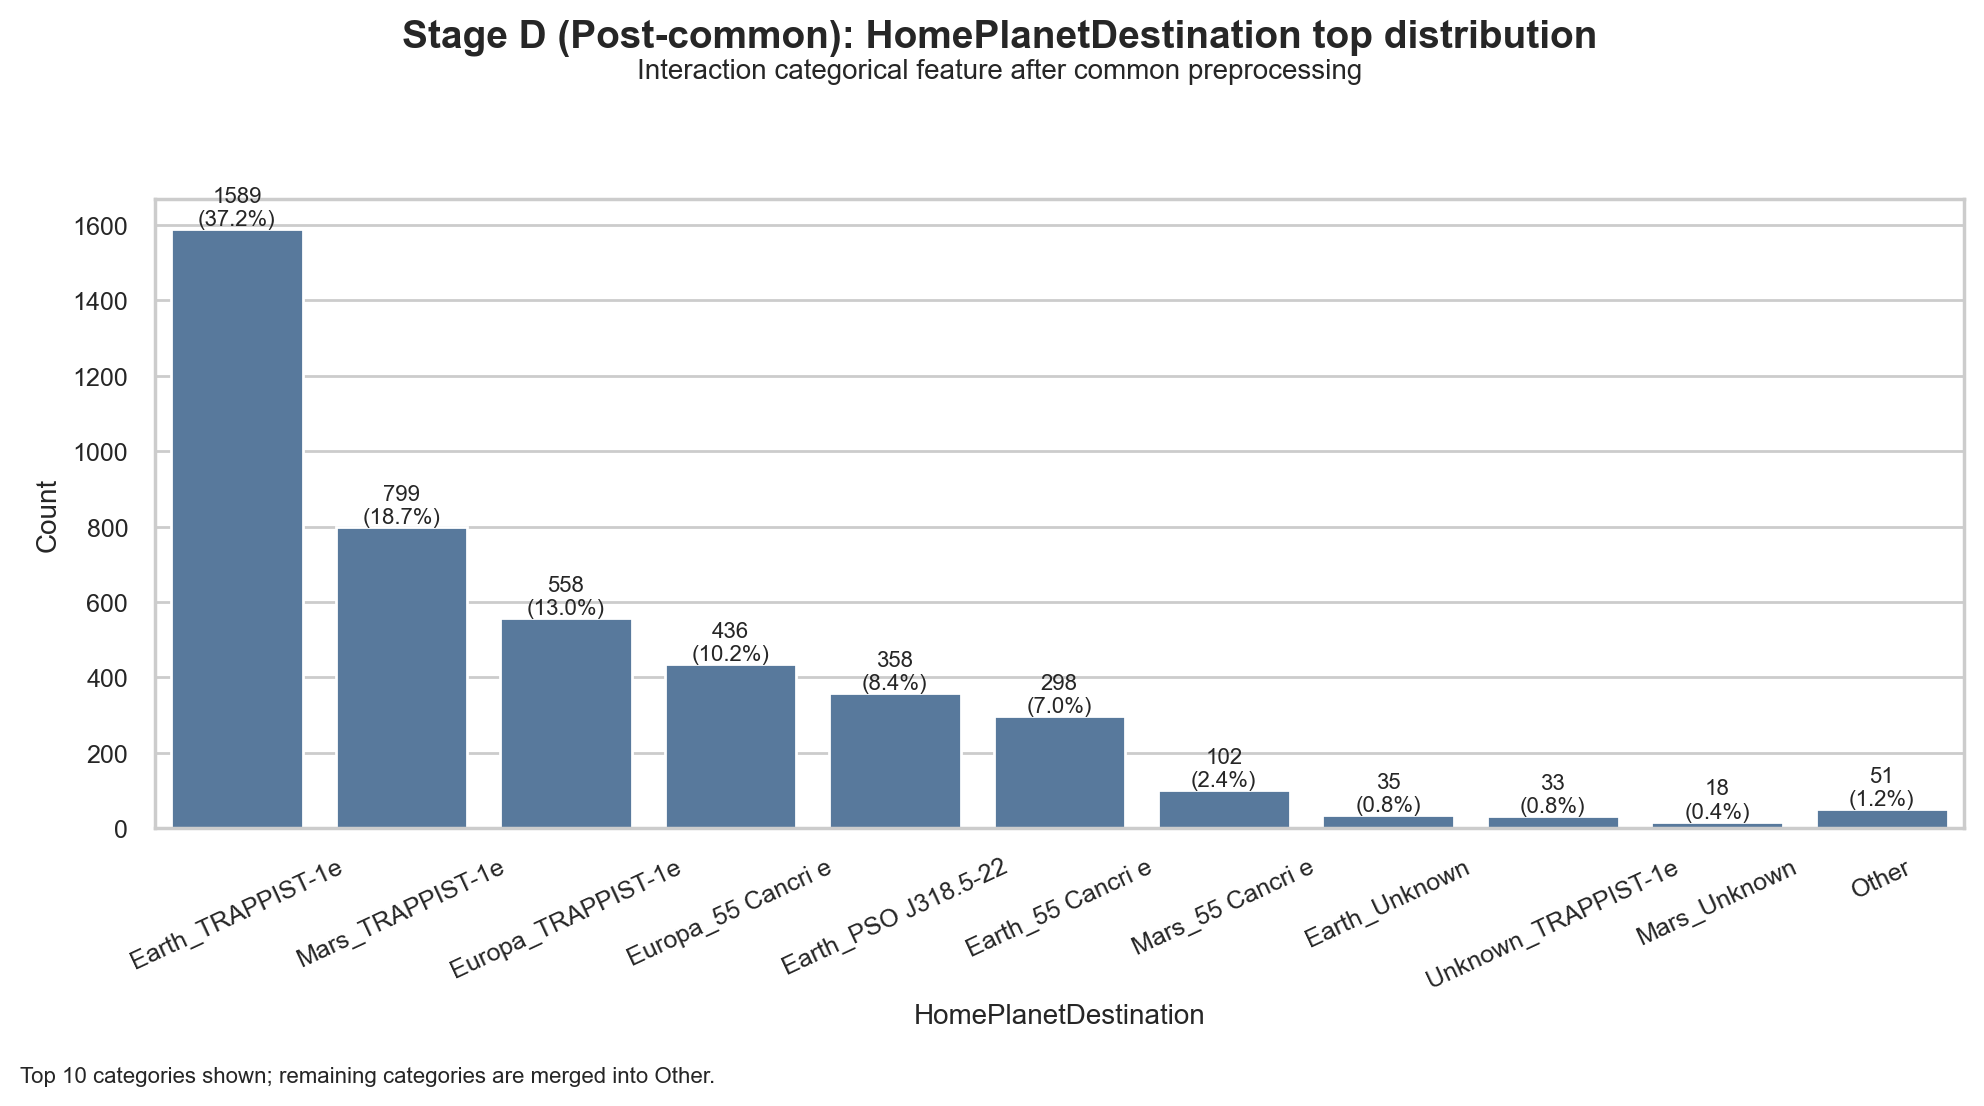
\includegraphics[width=\linewidth]{figures/eda/eda_homeplanet_destination_distribution.png}
\caption{Top HomePlanetDestination interaction categories after common preprocessing.}
\label{fig:eda_homeplanet_destination}
\end{figure}

The shared feature inventory can be summarized in five blocks: structural identifiers
(\texttt{PassengerId}, \texttt{GroupID}, \texttt{GroupMemberNo}, \texttt{GroupSize}, \texttt{Deck},
\texttt{CabinNum}, \texttt{Side}, \texttt{Surname}); common categorical fields
(\texttt{HomePlanet}, \texttt{CryoSleep}, \texttt{Destination}, \texttt{VIP}, \texttt{Deck}, \texttt{Side},
\texttt{AgeGroup}, \texttt{CabinNumBin}, \texttt{DeckSide}, \texttt{HomePlanetDestination}); base numeric
features (age, five spending columns, total-spend aggregates, group statistics, and binary flags); explicit
missingness indicators for the main raw columns; and CatBoost-only extra numeric/categorical features such as
\texttt{GroupMemberRatio}, \texttt{CabinNumLog1p}, \texttt{SpendStd}, \texttt{DeckCabinBin}, and
\texttt{SurnameFreqBin}.
This inventory deliberately treats missingness indicators and cross-field interactions as model inputs rather than as mere cleaning artifacts, which is consistent with recent analyses of supervised learning with incomplete tabular data~\cite{josse2024missingconsistency}.

\subsection{Branch-specific Representations}
After the common frame is finalized, each model receives a dedicated representation:
\begin{itemize}
\item Logistic Regression: \texttt{log1p} on spend-related features, numeric standardization, and one-hot encoded categorical variables.
\item Random Forest: raw numeric passthrough with one-hot encoded categoricals and no scaling.
\item XGBoost: \texttt{log1p} spend transforms plus one-hot encoded categoricals, but no scaling.
\item LightGBM: native pandas \texttt{category} columns with aligned train/test levels.
\item CatBoost: native string categorical columns, including \texttt{Surname}, plus branch-specific extra engineered features.
\end{itemize}
This branch-specific encoding choice is motivated by recent encoder benchmarks and tabular-model comparisons, which show that representation choice can materially change downstream ranking even when the learner family is held fixed~\cite{matteucci2023encoders,grinsztajn2022trees,mcelfresh2023nnsvstrees}.

This branch split is the exact place where the five models stop sharing a single feature representation.

In implementation terms, the five branches differ as follows. Logistic Regression applies \texttt{log1p} to
spend-related columns, standardizes the numeric block, one-hot encodes the categoricals, and fits a sparse
107-feature linear classifier. Random Forest keeps the engineered numeric values on their original scale,
one-hot encodes the same categorical block, and fits a sparse 107-feature tree ensemble. XGBoost also uses a
107-feature encoded matrix, but combines \texttt{log1p} numeric transforms with tree-based boosting rather than
scaling. This 107-feature XGBoost representation is the controlled local-validation baseline, not the final Kaggle-facing recovery submission. LightGBM keeps a 46-column DataFrame with aligned pandas categorical levels. CatBoost keeps a
62-column mixed-type DataFrame with extra engineered features and explicit categorical indices.

\begin{figure}[t]
\centering
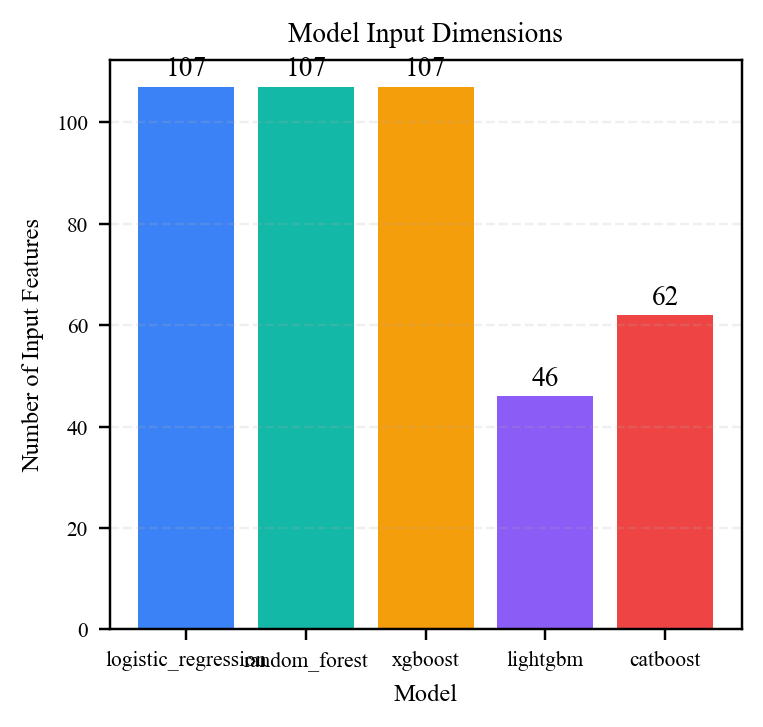
\includegraphics[width=\linewidth]{figures/model_input_dimensions.png}
\caption{Dimensionality of the baseline local-validation model inputs.}
\label{fig:model_input_dimensions}
\end{figure}

\section{Model Structures and Parameterization}
\subsection{Unified Structural View}
Although all five models solve the same binary classification problem, their internal structure is different. The project includes one linear probabilistic classifier, one bagged tree ensemble, and three gradient-boosted tree branches with different categorical-handling strategies. This mix is representative of modern strong baselines for heterogeneous tabular data~\cite{borisov2024tabularsurvey,grinsztajn2024betterdefault}.


\subsection{Logistic Regression}
The Logistic Regression branch uses a linear score and sigmoid probability:
\begin{align}
z_i &= w^\top x_i + b,\\
\hat{p}_i &= \sigma(z_i) = \frac{1}{1 + e^{-z_i}}.
\end{align}
The current validation baseline is implemented with \texttt{scikit-learn}~\cite{scikit_learn} and uses
\texttt{solver=lbfgs}, \texttt{C=1.0}, \texttt{max\_iter=1000}, and \texttt{random\_state=42}. In the lightweight search, the tuned best configuration was \texttt{C=0.01}, \texttt{penalty=l2}, \texttt{solver=lbfgs}, \texttt{max\_iter=1000}. This branch serves as the clearest linear baseline in the repository. Recent work shows that logistic-style models can remain useful when paired with interpretable feature engineering, while their interpretability still depends on feature coding, scaling, and user context rather than following automatically from the model name alone~\cite{rudin2019interpretable,dervovic2024logistic}.

\subsection{Random Forest}

Random Forest builds an ensemble of decision trees on bootstrapped samples~\cite{random_forest}. Each tree is trained on a randomly sampled subset of the training data, and different trees may learn different decision patterns. This design helps reduce the dependence on a single decision tree and improves the stability of the final prediction.

The output probability can be written as
\begin{equation}
\hat{p}_i = \frac{1}{T}\sum_{t=1}^{T} p_t(x_i),
\end{equation}
where $T$ is the number of trees, and $p_t(x_i)$ denotes the predicted probability produced by the $t$-th decision tree for sample $x_i$. The final probability $\hat{p}_i$ is obtained by averaging the probability outputs of all trees. Therefore, the final prediction is based on the collective decision of the whole forest rather than one individual tree.

The current validation baseline uses
\texttt{n\_estimators=400}, \texttt{max\_depth=None}, \texttt{min\_samples\_split=2}, \texttt{min\_samples\_leaf=1}, and \texttt{max\_features=sqrt}. Here, \texttt{n\_estimators=400} means that the model builds 400 decision trees. \texttt{max\_depth=None} allows each tree to grow until the stopping conditions are reached. \texttt{min\_samples\_split=2} means that a node can be split when it contains at least two samples, while \texttt{min\_samples\_leaf=1} allows each leaf node to contain at least one sample. The parameter \texttt{max\_features=sqrt} means that only a random subset of features is considered at each split, which increases diversity among trees and helps reduce overfitting~\cite{random_forest}.

Unlike Logistic Regression, Random Forest does not require feature scaling because decision trees split data according to feature thresholds rather than distance-based or gradient-based calculations. Therefore, the Random Forest branch keeps numerical features on their original scale and applies one-hot encoding to categorical variables. This remains consistent with recent tabular-learning comparisons that treat Random Forest as a strong out-of-the-box baseline, while noting that interpretation usually shifts from coefficients to importance-style summaries and variable-selection analysis~\cite{grinsztajn2022trees,rothacher2024rfvarselect}.

\subsection{XGBoost}
XGBoost is implemented as additive gradient-boosted trees~\cite{xgboost}:
\begin{equation}
F_M(x) = \sum_{m=1}^{M} \eta f_m(x),
\end{equation}
where $\eta$ is the learning rate and each $f_m$ is a regression tree. The training objective at boosting step $t$ is
\begin{equation}
\begin{aligned}
\mathcal{L}^{(t)}
    &= \sum_{i=1}^{n} l\left(y_i, \hat{y}_i^{(t-1)} + f_t(x_i)\right) \\
    &\quad + \Omega(f_t).
\end{aligned}
\end{equation}
The current baseline uses \texttt{n\_estimators=500}, \texttt{max\_depth=4}, \texttt{learning\_rate=0.05}, \texttt{subsample=0.9}, \texttt{colsample\_bytree=0.9}, and \texttt{tree\_method=hist}. This baseline configuration corresponds to the local validation comparison in Table~\ref{tab:baseline_results}.

Beyond this controlled validation baseline, XGBoost was maintained as a separate submission-oriented experimental branch. This branch used \texttt{StratifiedGroupKFold} to reduce passenger-group leakage, recomputed fold-dependent statistics such as \texttt{SurnameFreq} and \texttt{CabinNumBin} inside validation folds, and applied Optuna tuning after the validation design was leakage-aware. Earlier target-encoding variants produced inflated OOF scores and weaker public leaderboard behavior, so unsafe target-encoding features were removed from the clean XGBoost line. The final submitted file, \path{submission_team_common_rawlike_feedback_rank_k3_seed17_w05_true2291.csv}, was selected from documented submitted candidates and reached a Kaggle public leaderboard score of 0.81412. This score is reported as public submission evidence, not as a private-leaderboard or generalization guarantee~\cite{kapoor2024reforms}.

\subsection{LightGBM}
LightGBM follows the same additive boosting template~\cite{lightgbm},
\begin{equation}
F_t(x) = F_{t-1}(x) + \eta f_t(x),
\end{equation}
but the current implementation exploits two practical details:
\begin{itemize}
\item branch-specific native categorical columns are preserved as pandas \texttt{category} dtype,
\item train and test category levels are aligned before fitting.
\end{itemize}
\begin{table}[!t]
\caption{LightGBM top-feature configuration}
\label{tab:lightgbm_configuration}
\centering
\footnotesize
\begingroup
\setlength{\tabcolsep}{3pt}
\renewcommand{\arraystretch}{1.08}
\begin{tabularx}{\linewidth}{%
>{\raggedright\arraybackslash}p{0.22\linewidth}
>{\raggedright\arraybackslash}p{0.19\linewidth}
>{\raggedright\arraybackslash}p{0.22\linewidth}
Y}
\toprule
Setting & Value & Setting & Value \\
\midrule
Objective & \texttt{binary} & L1 reg. & \texttt{0.2} \\
Boosting type & \texttt{gbdt} & L2 reg. & \texttt{2.5} \\
Maximum budget & \texttt{5000 trees} & \texttt{max\_depth} & \texttt{-1} \\
Learning rate & \texttt{0.03} & Min split gain & \texttt{0.02} \\
Num. leaves & \texttt{23} & Subsample freq. & \texttt{1} \\
Min child samples & \texttt{40} & Final refit trees & \texttt{350} \\
Row subsample & \texttt{0.85} & Selected features & \texttt{30} \\
Column subsample & \texttt{0.75} & Best public LB & \texttt{0.80547} \\
\bottomrule
\end{tabularx}
\endgroup
\end{table}
The analyzed LightGBM top-feature branch uses the configuration summarized in Table~\ref{tab:lightgbm_configuration}. In the selected feature-ablation run, gain importance retained 30 features and the final refit used \texttt{n\_estimators=350}. This 30-feature setting is chosen because it has the best recorded Kaggle public leaderboard score, 0.80547, within the analyzed top-feature LightGBM branch, which is consistent with recent benchmark evidence that strong boosted-tree defaults remain highly competitive on tabular tasks~\cite{grinsztajn2024betterdefault,salinas2024tabrepo}.
Native handling of aligned categorical columns is one reason this branch remains competitive on heterogeneous tabular data and in data-centric benchmark settings~\cite{matteucci2023encoders,grinsztajn2022trees,tschalzev2024datacentric}.

\subsection{CatBoost}
CatBoost is also an additive tree model~\cite{catboost}, but it is particularly suited to mixed numeric and categorical tabular inputs. The implementation in this project keeps categorical columns as strings and passes the column indices explicitly to the learner. The decision to retain \texttt{Surname} and related categorical interactions in this branch follows recent work showing that high-cardinality categorical fields can be useful when the model family is designed to absorb them directly~\cite{matteucci2023encoders,avanzi2023highcardinality}. The baseline uses \texttt{iterations=500}, \texttt{depth=6}, \texttt{learning\_rate=0.05}, \texttt{loss\_function=Logloss}, \texttt{eval\_metric=Accuracy}, and \texttt{random\_seed=42}.

\section{Optimization and Validation Design}
\subsection{Project-side Training Scripts}
The repository contains both the lightweight validation layer and standalone model-training scripts. The validation layer is designed for controlled comparison; the training scripts are closer to the actual submission workflow. Two operations recur across these scripts:
\begin{equation}
\hat{y}_i(\tau) = \mathbb{1}[\hat{p}_i \ge \tau],
\end{equation}
which defines thresholded classification, and, for multi-seed ensembles,
\begin{equation}
\bar{p}_i = \frac{1}{S}\sum_{s=1}^{S} \hat{p}_i^{(s)},
\end{equation}
which averages predicted probabilities over $S$ random seeds before thresholding.
Choosing $\tau$ on out-of-fold or held-out probabilities is consistent with recent threshold-optimization and calibration guidance, provided the threshold is selected inside the validation loop rather than on the final test split~\cite{silva2023calibration,lee2023tcal,leevy2023threshold,kapoor2023leakage}.

The project-side training scripts are more specialized than the lightweight validation layer. Logistic Regression fits the frozen sparse LR bundle with \texttt{solver=saga}, \texttt{penalty=l2}, \texttt{C=1.0}, and fixed threshold $\tau=0.5$, whereas Random Forest uses a tuned high-capacity recipe (\texttt{n\_estimators=2600}, \texttt{max\_depth=16}, \texttt{criterion=log\_loss}, \texttt{class\_weight=balanced}) and stores an accuracy-optimized OOF threshold. The XGBoost submission branch is handled separately from the lightweight validation layer because it has its own group-aware CV, fold-aware preprocessing, Optuna search, ablation, leak diagnosis, SHAP/importance, multi-seed bagging, and final submission-selection workflow. LightGBM uses 5-fold \texttt{StratifiedKFold} CV, 250-round early stopping on validation \texttt{binary\_logloss}, OOF-based threshold tuning, and a final refit with the selected 30-feature subset and \texttt{n\_estimators=350}. CatBoost uses \texttt{iterations=2000}, \texttt{learning\_rate=0.03}, \texttt{depth=6}, \texttt{l2\_leaf\_reg=5.0}, and 5-fold CV with OOF threshold search in its \texttt{cv\_tune} mode.

\subsection{Holdout Validation Protocol}
The current comparison uses a stratified holdout split:
\begin{equation}
\begin{aligned}
(\mathcal{D}_{\mathrm{train}}, \mathcal{D}_{\mathrm{valid}})
&= \operatorname{Split}_{0.8/0.2}(\mathcal{D}; \\
&\quad \texttt{random\_state}=42, \\
&\quad \texttt{stratify}=\texttt{Transported}).
\end{aligned}
\label{eq:holdout_split}
\end{equation}
This produces 6954 local training rows and 1739 local validation rows. All train-fit preprocessing statistics are then recomputed on the local training partition only, which is essential for leakage control and for making the resulting model comparison reproducible~\cite{kapoor2023leakage,kapoor2024reforms}.

\subsection{Metrics}
The validation runner records
\texttt{accuracy}, \texttt{precision}, \texttt{recall}, \texttt{F1}, \texttt{ROC-AUC}, \texttt{fit\_seconds}, and \texttt{predict\_seconds}. Accuracy is the primary ranking metric, but it is not the only one retained because threshold quality, ranking quality, and probability calibration answer different evaluation questions~\cite{silva2023calibration,lee2023tcal}. This is why the project also keeps ROC curves, probability distributions, calibration plots, and threshold sweeps rather than reporting a single thresholded score~\cite{leevy2023threshold}.

\subsection{Hyperparameter Search Spaces}
The validation layer implements a lightweight tuning module. The current lightweight tuning table covers Logistic Regression, Random Forest, LightGBM, and CatBoost. XGBoost has a baseline validation configuration in Table~\ref{tab:baseline_parameters}, while its stronger local experiments are tracked in the separate XGBoost module rather than in this lightweight cross-model tuning snapshot.

\begin{table}[!t]
\caption{Exact baseline parameters and current LightGBM setting}
\label{tab:baseline_parameters}
\centering
\footnotesize
\begingroup
\setlength{\tabcolsep}{3pt}
\renewcommand{\arraystretch}{1.08}
\begin{tabularx}{\linewidth}{%
>{\raggedright\arraybackslash}p{0.23\linewidth}
Y}
\toprule
Model & Exact configuration in the current validation layer \\
\midrule
Logistic Regression & \texttt{max\_iter=1000}, \texttt{solver=lbfgs}, \texttt{C=1.0}, \texttt{random\_state=42}. \\
Random Forest & \texttt{n\_estimators=400}, \texttt{max\_depth=None}, \texttt{min\_samples\_split=2}, \texttt{min\_samples\_leaf=1}, \texttt{max\_features=sqrt}, \texttt{n\_jobs=-1}, \texttt{random\_state=42}. \\
XGBoost & \texttt{n\_estimators=500}, \texttt{max\_depth=4}, \texttt{learning\_rate=0.05}, \texttt{subsample=0.9}, \texttt{colsample\_bytree=0.9}, \texttt{eval\_metric=logloss}, \texttt{tree\_method=hist}, \texttt{n\_jobs=-1}, \texttt{random\_state=42}. \\
LightGBM & \texttt{objective=binary}, \texttt{boosting\_type=gbdt}, \texttt{n\_estimators=5000}, \texttt{learning\_rate=0.03}, \texttt{num\_leaves=23}, \texttt{min\_child\_samples=40}, \texttt{subsample=0.85}, \texttt{colsample\_bytree=0.75}, \texttt{reg\_alpha=0.2}, \texttt{reg\_lambda=2.5}, \texttt{max\_depth=-1}, \texttt{min\_split\_gain=0.02}, \texttt{subsample\_freq=1}, \texttt{n\_jobs=-1}. \\
CatBoost & \texttt{iterations=500}, \texttt{depth=6}, \texttt{learning\_rate=0.05}, \texttt{loss\_function=Logloss}, \texttt{eval\_metric=Accuracy}, \texttt{verbose=False}, \texttt{allow\_writing\_files=False}, \texttt{random\_seed=42}. \\
\bottomrule
\end{tabularx}
\endgroup
\end{table}

The lightweight validation search spaces are deliberately small. Logistic Regression tunes only \texttt{C}
over $\{0.01,0.1,1.0,3.0,10.0\}$. Random Forest varies tree count, depth, split thresholds, leaf size, and
\texttt{max\_features}.
LightGBM uses the tuned parameter set reported above for the current top-feature run; this run did not rerun random hyperparameter search. Its threshold search uses OOF probabilities over the grid $[0.44,0.54]$ with step $0.005$ and selects the threshold that maximizes CV accuracy. CatBoost varies iteration budget, depth, learning rate, and \texttt{l2\_leaf\_reg}. This intentionally small search design reflects recent evidence that strong pre-tuned defaults can already be competitive on tabular benchmarks, especially when the feature representation is stable and the evaluation loop is well controlled~\cite{grinsztajn2024betterdefault,salinas2024tabrepo}.

\begin{table}[t]
\caption{Current tuning outcomes recorded in the repository}
\label{tab:tuning_outcomes}
\centering
\footnotesize
\begingroup
\setlength{\tabcolsep}{2.5pt}
\renewcommand{\arraystretch}{1.16}
\begin{tabularx}{\linewidth}{%
>{\raggedright\arraybackslash}p{0.17\linewidth}
>{\raggedright\arraybackslash}p{0.22\linewidth}
>{\centering\arraybackslash}p{0.13\linewidth}
Y}
\toprule
Model & Search setup & Best CV score & Best parameters \\
\midrule
Logistic Regression
& 3-fold random search, 5 trials
& 0.7866
& \texttt{C=0.01}; \texttt{max\_iter=1000}; \texttt{penalty=l2}; \texttt{solver=lbfgs}. \\
Random Forest
& 3-fold random search, 5 trials
& 0.8069
& \texttt{max\_depth=14}; \texttt{max\_features=sqrt}; \texttt{min\_samples\_leaf=2}; \texttt{min\_samples\_split=10}; \texttt{n\_estimators=200}. \\
XGBoost
& Not included in this lightweight tuning snapshot
& 0.8223
& Maintained separately through the dedicated XGBoost validation and submission workflow. \\
LightGBM
& 5-fold top-feature refit, 1 selected run
& 0.8177
& \texttt{learning\_rate=0.03}; \texttt{num\_leaves=23}; \texttt{min\_child\_samples=40}; \texttt{subsample=0.85}; \texttt{colsample\_bytree=0.75}; \texttt{reg\_alpha=0.2}; \texttt{reg\_lambda=2.5}; \texttt{threshold=0.500}; \texttt{final\_n\_estimators=350}; \texttt{selected\_features=30}. \\
CatBoost
& 3-fold random search, 5 trials
& 0.8138
& \texttt{depth=6}; \texttt{iterations=800}; \texttt{l2\_leaf\_reg=1}; \texttt{learning\_rate=0.05}. \\
\bottomrule
\end{tabularx}
\endgroup
\end{table}

\noindent The dash in the XGBoost row refers only to this lightweight cross-model tuning snapshot. It does not mean
that the XGBoost branch was absent or untuned; that branch was maintained separately with a dedicated
\texttt{StratifiedGroupKFold}, fold-aware preprocessing, Optuna-based tuning, ablation, leak diagnosis, and
submission-selection workflow. Therefore, Table~\ref{tab:tuning_outcomes} should be read as the shared lightweight
tuning summary, while the XGBoost-specific evidence is reported as a separate final-submission branch.

\section{Results}
\subsection{Baseline Validation Results}
Table~\ref{tab:baseline_results} summarizes the baseline validation run \texttt{validation\_001}. The selected LightGBM top-feature run is reported separately because it uses 5-fold OOF CV and feature-ablation refitting rather than the single holdout validation layer.

\begin{table}[t]
\caption{Baseline local validation results}
\label{tab:baseline_results}
\centering
\footnotesize
\resizebox{\linewidth}{!}{%
\begin{tabular}{lccccccc}
\toprule
Model & Accuracy & Precision & Recall & F1 & ROC-AUC & Fit (s) & Predict (s) \\
\midrule
LightGBM & 0.8171 & 0.8178 & 0.8196 & 0.8187 & 0.9095 & 1.6837 & 0.0383 \\
CatBoost & 0.8154 & 0.8129 & 0.8231 & 0.8179 & 0.9125 & 44.4018 & 0.0398 \\
XGBoost & 0.8114 & 0.8079 & 0.8208 & 0.8143 & 0.9119 & 1.0165 & 0.0221 \\
Random Forest & 0.8091 & 0.8269 & 0.7854 & 0.8056 & 0.9038 & 0.8591 & 0.2625 \\
Logistic Regression & 0.7907 & 0.7783 & 0.8174 & 0.7973 & 0.8790 & 0.5503 & 0.0132 \\
\bottomrule
\end{tabular}
}
\end{table}

The baseline result table already provides the full numeric ranking. The standalone accuracy bar chart is moved to
the appendix to keep the main paper layout compact. Under this local validation protocol, XGBoost ranks behind LightGBM and CatBoost by accuracy, but remains competitive in ROC-AUC and runtime. This statement refers only to the local validation layer; the later Kaggle public result should not be used to reorder the local validation ranking.

\begin{table}[t]
\caption{Selected LightGBM top-feature run}
\label{tab:lightgbm_top_feature}
\centering
\footnotesize
\begingroup
\setlength{\tabcolsep}{4pt}
\renewcommand{\arraystretch}{1.16}
\begin{tabularx}{\linewidth}{l Y}
\toprule
Item & Value \\
\midrule
Model & LightGBM top-feature \\
Selected features & 30 \\
CV accuracy at threshold 0.5 & 0.8177 \\
Tuned CV accuracy & 0.8177 \\
Best threshold & 0.500 \\
Final trees & 350 \\
\bottomrule
\end{tabularx}
\endgroup
\end{table}

\subsection{Overall Model Comparison}

Table~\ref{tab:overall_model_comparison} summarizes the training accuracy, local validation accuracy,
local validation ROC-AUC, and retained Kaggle public leaderboard evidence for the five evaluated models.
The table should be interpreted along two separate axes: local validation performance and external public
leaderboard feedback.

\begin{table*}[t]
\caption{Overall comparison of local validation performance and retained Kaggle public leaderboard evidence}
\label{tab:overall_model_comparison}
\centering
\footnotesize
\resizebox{0.86\textwidth}{!}{%
\begin{tabular}{lcccc}
\toprule
Model & Train Accuracy & Validation Accuracy & Validation ROC-AUC & Retained Public LB Evidence \\
\midrule
XGBoost & 0.8834 & 0.8114 & 0.9119 & 0.81412 \\
CatBoost & 0.8622 & 0.8154 & 0.9125 & Not retained \\
LightGBM & 0.9617 & 0.8171 & 0.9095 & 0.80547 \\
Random Forest & 1.0000 & 0.8091 & 0.9038 & Not retained \\
Logistic Regression & 0.7916 & 0.7907 & 0.8790 & Not retained \\
\bottomrule
\end{tabular}
}
\end{table*}

The results show that the strongest model depends on the evaluation dimension. LightGBM obtains the
highest local validation accuracy, reaching 0.8171, which indicates the best thresholded classification
performance on the local holdout split. CatBoost obtains the highest validation ROC-AUC, reaching 0.9125,
which suggests that its probability ranking quality is slightly stronger than the other models under the
same local validation setting. However, the strongest retained Kaggle public leaderboard evidence comes from the
XGBoost branch, with a retained public score of 0.81412. The package also retains the analyzed LightGBM
top-feature branch public score of 0.80547. Other historical CatBoost, Random Forest, and Logistic Regression
public-score records are not used as package evidence because their original leaderboard screenshots or
submission records were not preserved in the final evidence folder.

This distinction is important because local validation metrics and Kaggle public leaderboard scores measure
different forms of evidence. The local validation scores are produced under the controlled holdout protocol,
whereas the public leaderboard scores reflect external feedback from submitted prediction files. Therefore,
LightGBM can be described as the local validation accuracy leader, CatBoost as the local ROC-AUC leader, and
XGBoost as the strongest retained public leaderboard submission in the current workspace.

The training accuracy column also helps diagnose overfitting. Random Forest reaches 1.0000 training accuracy
but only 0.8091 validation accuracy, indicating clear overfitting despite competitive validation performance.
LightGBM also shows a large train-validation gap, although it still achieves the best local validation
accuracy. In contrast, Logistic Regression has much closer train and validation accuracy, but its lower ROC-AUC
indicates limited model capacity for this feature representation.

\subsection{Threshold-independent and Threshold-dependent Behavior}
The current project already stores per-sample validation probabilities, which makes threshold-independent analysis possible through ROC curves and threshold-dependent analysis possible through threshold sweeps. The large multi-panel threshold figures are moved to the appendix so they do not break the main paper layout.

\begin{figure}[t]
\centering
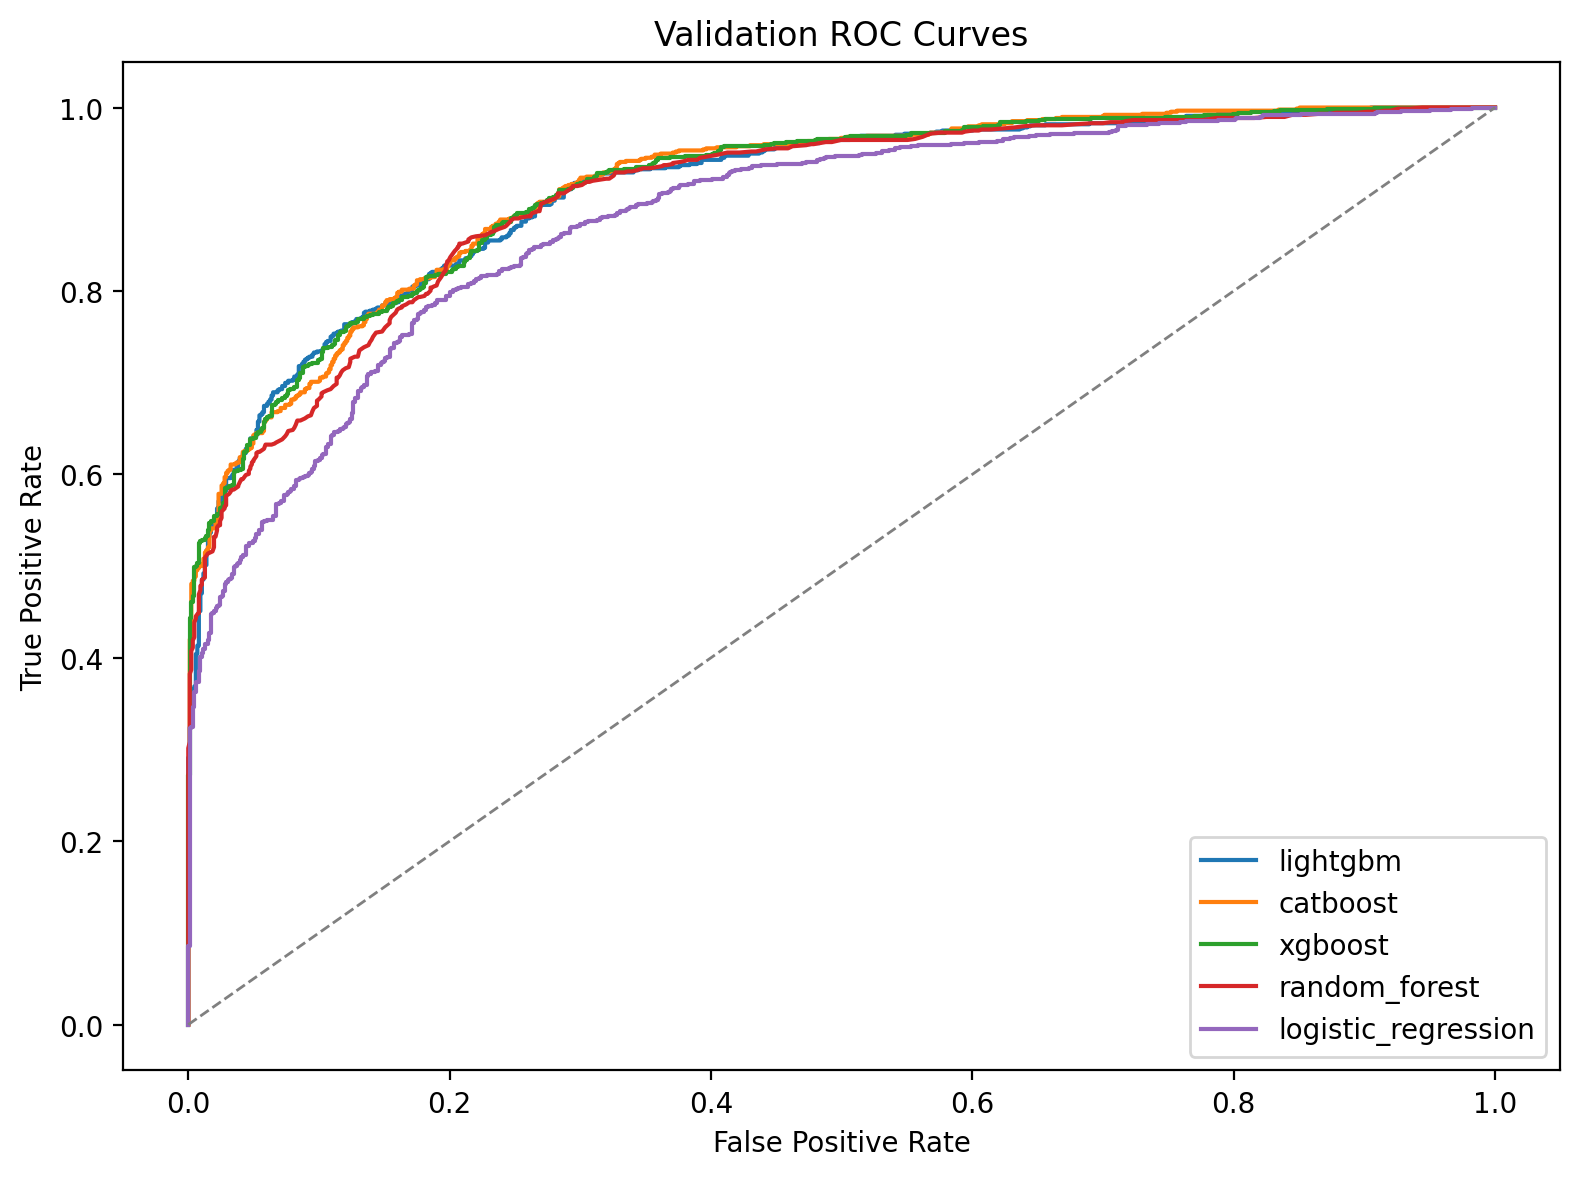
\includegraphics[width=\linewidth]{figures/validation_roc_curves.png}
\caption{ROC curves across all models.}
\label{fig:roc_curves}
\end{figure}

\subsection{Error and Runtime Analysis}
The project also includes side-by-side confusion matrices and runtime plots. The multi-panel confusion-matrix figure
and the standalone runtime comparison chart are moved to the appendix so that the main text keeps a more compact
narrative flow.

\subsection{Optimization Impact}
Lightweight tuning does not uniformly improve all models. This is a meaningful experimental result in itself: for
the current feature branches, branch design and leakage-aware preprocessing appear to matter at least as much as
shallow random search. Additional package figures, including calibration curves, precision-recall curves,
probability histograms, runtime trade-off plots, boosting-iteration proxies, and tuned-versus-baseline charts,
are retained in the report folder but omitted from the main paper body to keep float pressure manageable. This interpretation is consistent with recent data-centric benchmark work showing that preprocessing and representation choices can dominate marginal hyperparameter gains on tabular tasks~\cite{tschalzev2024datacentric,grinsztajn2024betterdefault}.

\subsection{Feature Interpretation}
The project provides both per-model importance plots and a normalized cross-model heatmap. This is important because raw importance values are not directly comparable across linear, bagged-tree, and boosting models, and because different importance definitions can lead to different selected subsets or narratives~\cite{lundberg2017shap,strobl2007bias,rothacher2024rfvarselect}.
The normalized heatmap is retained in the appendix together with other supplementary diagnostics.

\section{Kaggle Submission Table}
The Kaggle table reports retained public leaderboard evidence for the part covered here. Public scores are listed only when the package preserves a corresponding screenshot, submission file, metadata record, or branch-level evidence. These public scores are external submission feedback and are not interpreted as private-leaderboard guarantees. Keeping leaderboard evidence separate from controlled local validation follows current guidance on more reproducible machine-learning reporting~\cite{kapoor2024reforms}.

\begin{table}[H]
\caption{Kaggle public leaderboard evidence for selected submissions}
\label{tab:kaggle_scores}
\centering
\footnotesize
\begingroup
\setlength{\tabcolsep}{4pt}
\renewcommand{\arraystretch}{1.16}
\begin{tabularx}{\linewidth}{%
>{\raggedright\arraybackslash}p{0.19\linewidth}
>{\centering\arraybackslash}p{0.18\linewidth}
Y}
\toprule
Model &  Public LB & Notes \\
\midrule
XGBoost
& 0.81412
& Private LB not claimed; documented final XGBoost public submission. \\
LightGBM
& 0.80547
& Private LB not claimed; best recorded public score within the analyzed top-feature LightGBM branch. \\
\bottomrule
\end{tabularx}
\endgroup
\end{table}

Historical public-score notes without retained package evidence are not used in this table. Therefore,
CatBoost, Random Forest, and Logistic Regression are compared through the controlled local validation columns
in Table~\ref{tab:overall_model_comparison}, while the retained public-score evidence is limited to XGBoost
and the analyzed LightGBM top-feature branch.

\begin{figure}[t]
\centering
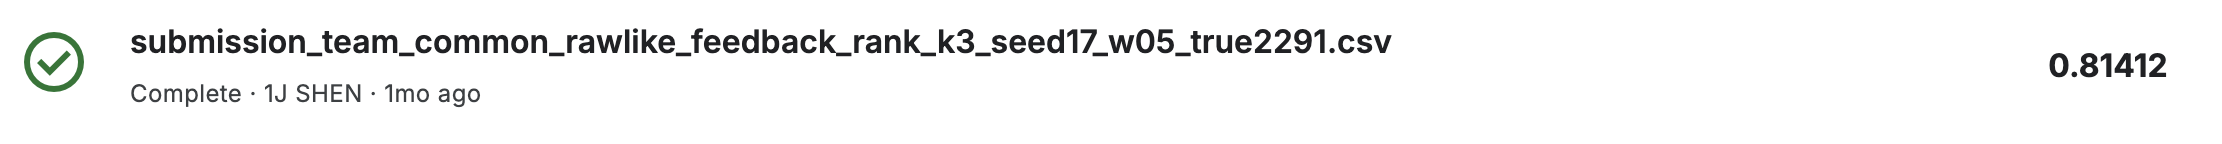
\includegraphics[width=\linewidth]{figures/kaggle_best_submission_score.png}
\caption{Kaggle public leaderboard feedback for the best recorded team submission. The screenshot shows the submitted file \texttt{submission\_team\_common\_rawlike\_feedback\_rank\_k3\_seed17\_w05\_true2291.csv} with a public score of 0.81412. This evidence is used only as public leaderboard feedback and is not interpreted as a private-leaderboard guarantee.}
\label{fig:kaggle_best_submission}
\end{figure}

Figure~\ref{fig:kaggle_best_submission} records the external Kaggle feedback for the best team submission used in this report.
\textbf{Code Availability.} The project code is available at \url{https://github.com/u430034056-tech/epoch-MLW.git}. The submitted ZIP package also includes a source-code snapshot and local reproduction scripts for offline inspection.

Across all recorded LightGBM submissions in the repository, the highest public leaderboard score is 0.80710 from \texttt{submission\_lightgbm\_no\_rule.csv}; however, the present report focuses on the separately analyzed top-feature LightGBM branch, whose best recorded public score is 0.80547.

\section{Discussion}
Several implementation-driven observations are worth emphasizing:
\begin{itemize}
\item The preprocessing layer is not generic boilerplate; it encodes domain-motivated rules such as CryoSleep zero-spend enforcement, group-consistent category completion, and train-only surname frequency mapping, which is closer to a data-centric tabular workflow than to a purely model-centric one~\cite{chicco2022tips,kapoor2023leakage,tschalzev2024datacentric}.
\item LightGBM benefits from a compact branch with native categorical handling; the selected 30-feature gain-ranked run achieves a tuned 5-fold CV accuracy of 0.8177 and the best recorded public leaderboard score of 0.80547 within the analyzed top-feature LightGBM branch, consistent with recent evidence that strong tree-based defaults remain hard to beat on typical tabular tasks~\cite{grinsztajn2022trees,grinsztajn2024betterdefault}.
\item CatBoost benefits from retaining \texttt{Surname} and other high-cardinality categorical signals directly, but this comes with much higher training time~\cite{matteucci2023encoders,avanzi2023highcardinality}.
\item XGBoost is not the strongest local-validation model by accuracy, but it remains competitive in ROC-AUC and runtime. Its main contribution is a separate validated submission branch with group-aware validation, fold-aware feature recomputation, Optuna tuning, leak diagnosis, SHAP/importance evidence, multi-seed bagging, and a documented final public submission score of 0.81412.
\item Logistic Regression is the weakest model by raw score but remains a useful linear baseline; its interpretability should still be understood as relative rather than automatic~\cite{dervovic2024logistic}.
\end{itemize}

\section{Limitations and Future Work}
This study has several limitations:
\begin{itemize}
\item The local model comparison currently relies on a single stratified holdout rather than repeated cross-validation.
\item The full preprocessing layer uses combined train+test group size for final bundle generation, which is acceptable for inference-oriented preprocessing but must remain split-local during validation.
\item XGBoost is not included in the shared lightweight tuning snapshot; its dedicated Optuna tuning, ablation, and final submission branch are therefore reported separately from Table~\ref{tab:tuning_outcomes}.
\item Full per-iteration convergence histories are not persisted by the validation runner.
\item The reported XGBoost and LightGBM public leaderboard scores are external submission feedback and should not be treated as private-leaderboard guarantees.
\item The final XGBoost file was selected using documented Kaggle public feedback; this should be described as final submission selection, not as proof that a public-feedback perturbation is a generally superior modeling method.
\end{itemize}

Immediate next steps for the XGBoost branch include repeated cross-validation, broader XGBoost tuning under the same validation protocol, and additional Kaggle submissions only if new XGBoost candidates are actually submitted. More broadly, future work could evaluate stronger missing-data pipelines such as automatic model-selection-based imputation, compare against modern deep tabular baselines, and place the current workflow in a larger repository-style benchmark context~\cite{jarrett2022hyperimpute,somvanshi2024deeptabular,salinas2024tabrepo,kapoor2024reforms}.

\section{Contribution Statement}
All five team members contributed equally to the project. Each member's contribution is assigned as 20\% of the total work. The detailed division of work is summarized in Table~\ref{tab:team_contribution}.

\begin{table}[H]
\caption{Team contribution statement}
\label{tab:team_contribution}
\centering
\scriptsize
\begin{tabularx}{\columnwidth}{>{\raggedright\arraybackslash}p{0.23\columnwidth}Y>{\centering\arraybackslash}p{0.12\columnwidth}}
\toprule
Member & Main responsibilities & Share \\
\midrule
Wang Han & Logistic Regression feature engineering and model construction; report writing and integration; PPT production. & 20\% \\
Shen Yijie & Shared data preprocessing; XGBoost feature engineering and model construction; report writing and integration; PPT production; overall project integration and local reproduction. & 20\% \\
Yang Yusong & Exploratory data analysis; LightGBM feature engineering and model construction; report writing and integration; PPT production. & 20\% \\
Jiang Zhibo & Exploratory data analysis; Random Forest feature engineering and model construction; report writing and integration; PPT production. & 20\% \\
He Yuxiang & CatBoost preprocessing, feature engineering, and model construction; report writing and integration; PPT production and integration. & 20\% \\
\bottomrule
\end{tabularx}
\end{table}

\section{Conclusion}
This study developed a leakage-aware preprocessing and validation workflow for the Spaceship Titanic classification task and compared five supervised tabular models under a common evaluation protocol. The local evidence is metric-dependent: LightGBM leads local validation accuracy, CatBoost leads ROC-AUC, and XGBoost is the final branch with the strongest recorded public leaderboard submission. For final external submission feedback, the selected XGBoost branch reached a Kaggle public leaderboard score of 0.81412. The main remaining limitation is that the cross-model comparison still relies on a single stratified holdout split rather than repeated cross-validation, which should be addressed in future work.

\appendices
\section{Supplementary Figures}
Large diagnostic figures are collected here so the main body stays readable while the supporting plots remain available for inspection.

\begin{figure}[t]
\centering
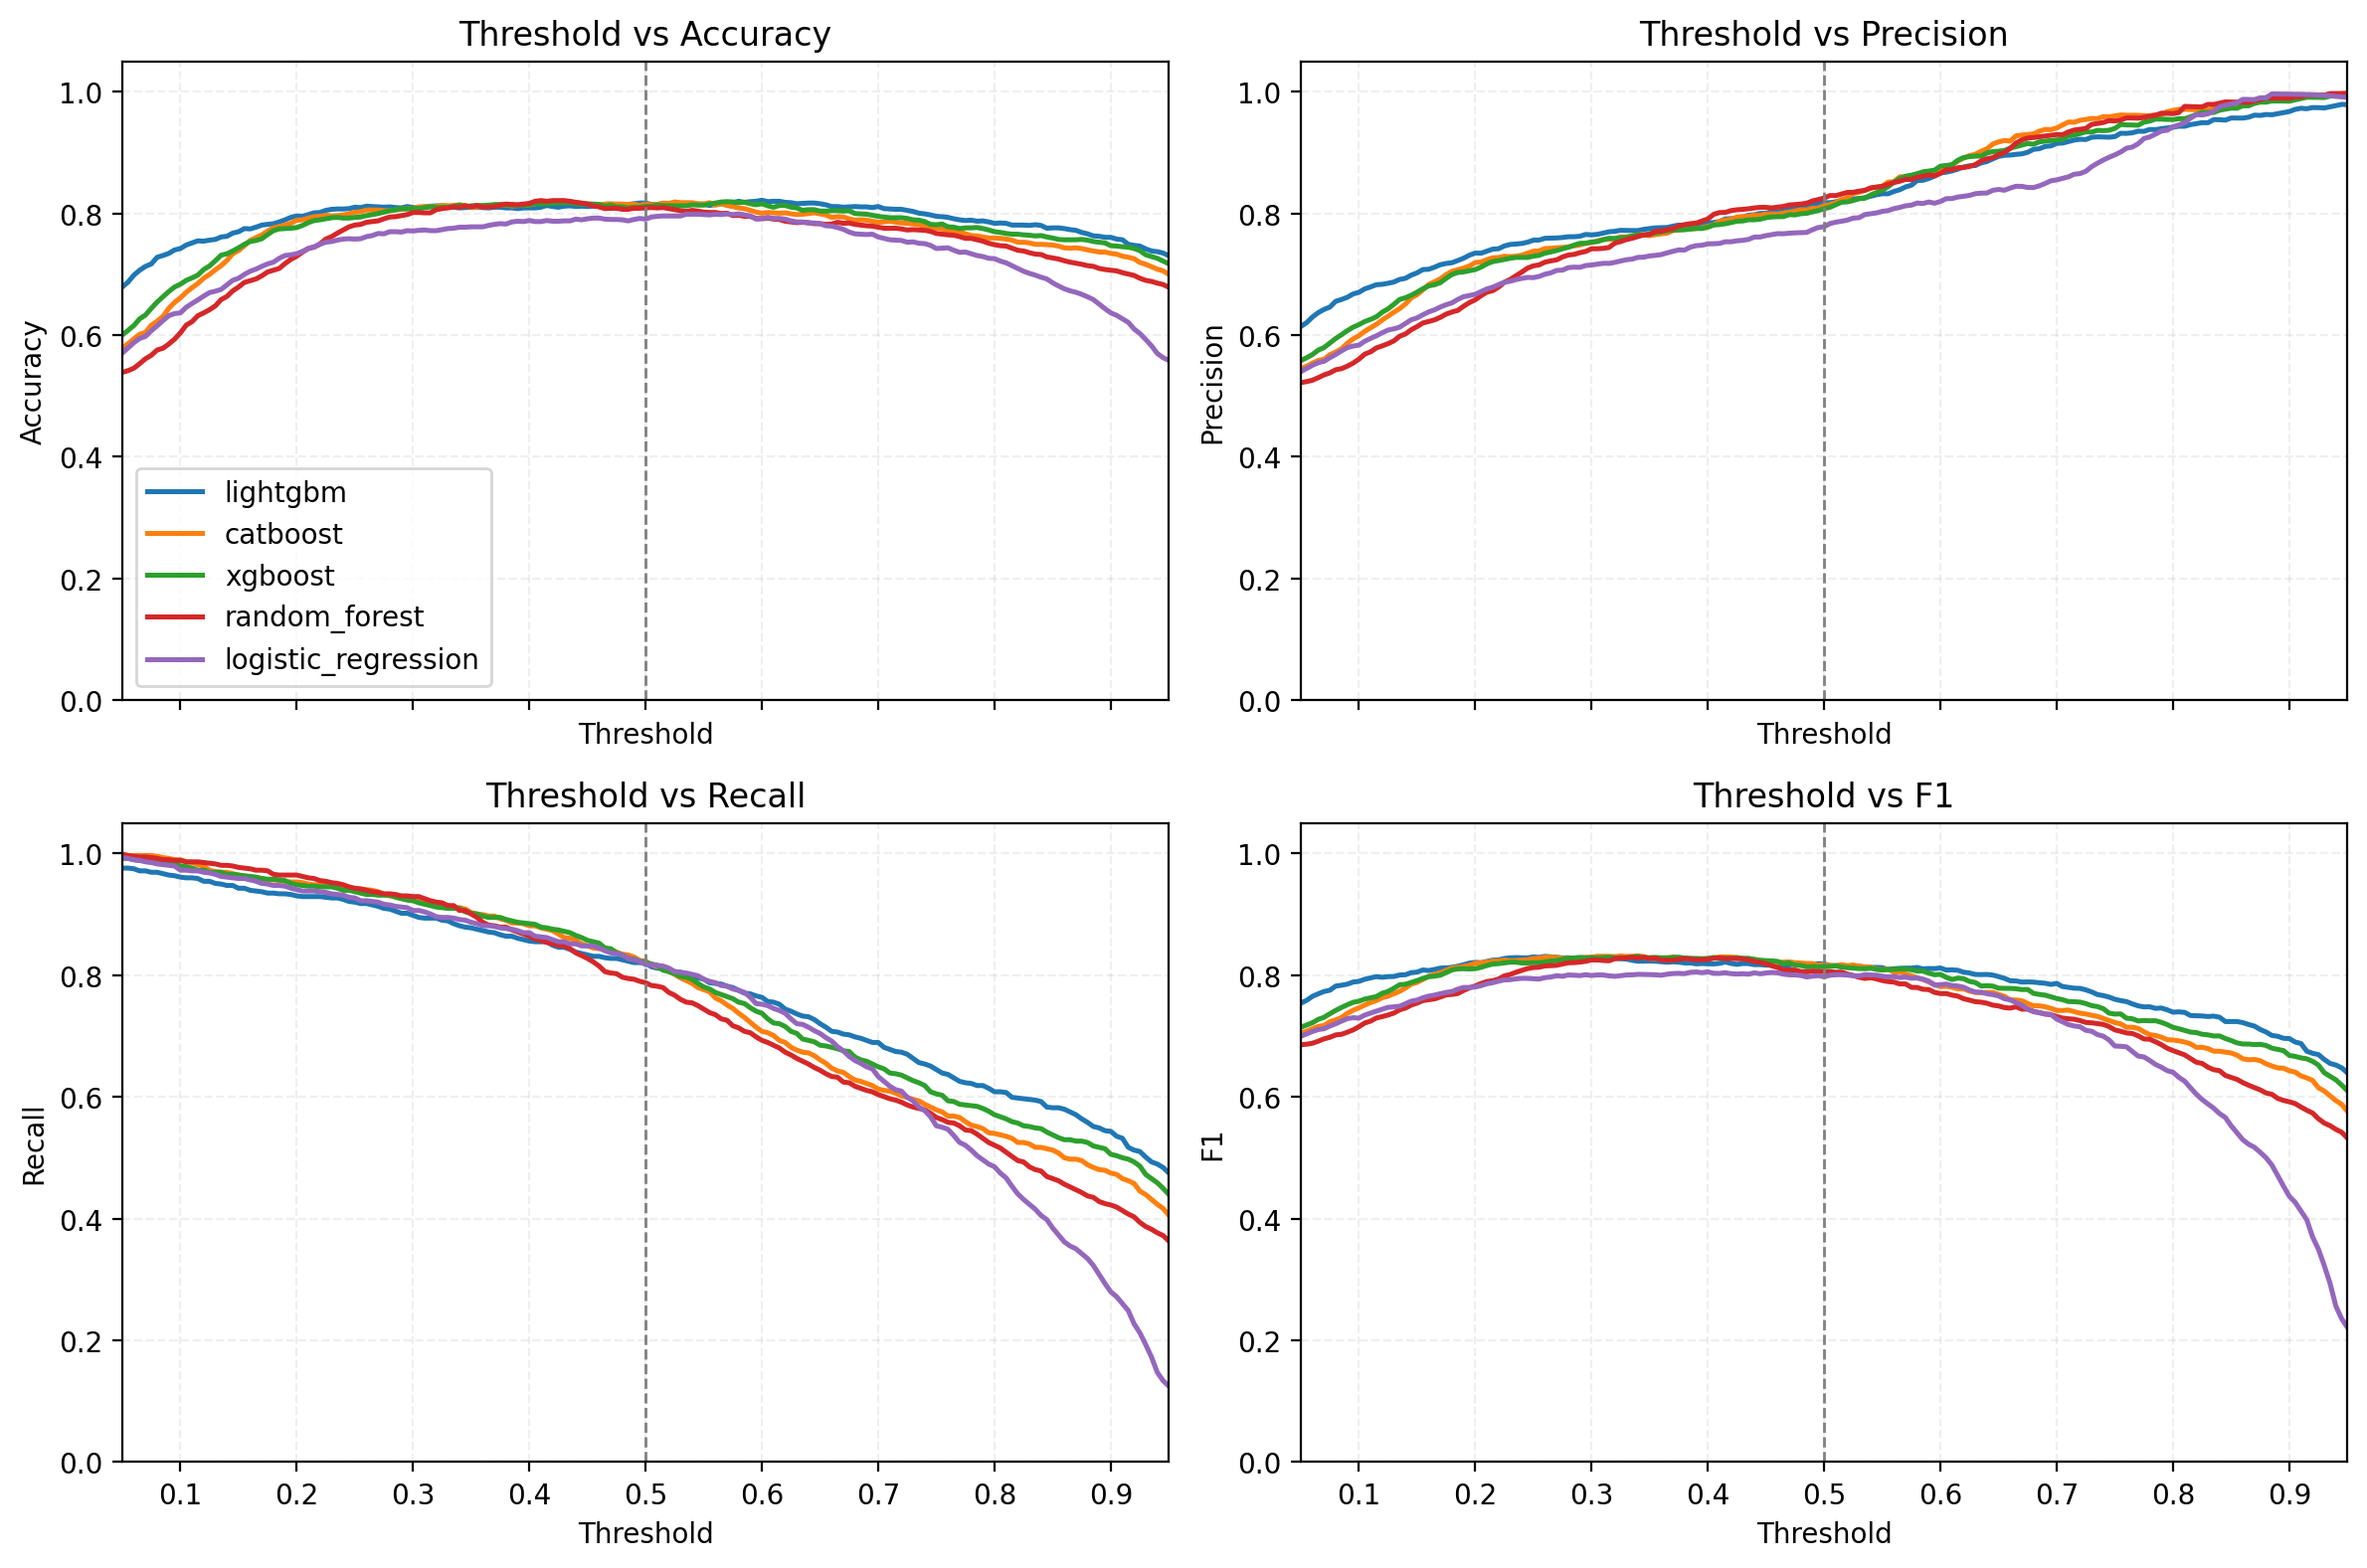
\includegraphics[width=\linewidth]{figures/validation_threshold_metric_overlays.png}
\caption{Global threshold overlays for accuracy, precision, recall, and F1 across the five evaluated models on the local validation split. Accuracy and F1 remain relatively stable in the mid-threshold region, while precision increases and recall decreases as the decision threshold becomes more conservative. The dashed vertical line at 0.5 marks the default threshold and shows that it provides a reasonable overall trade-off without model-specific threshold tuning.}
\label{fig:threshold_global}
\end{figure}

\begin{figure}[t]
\centering
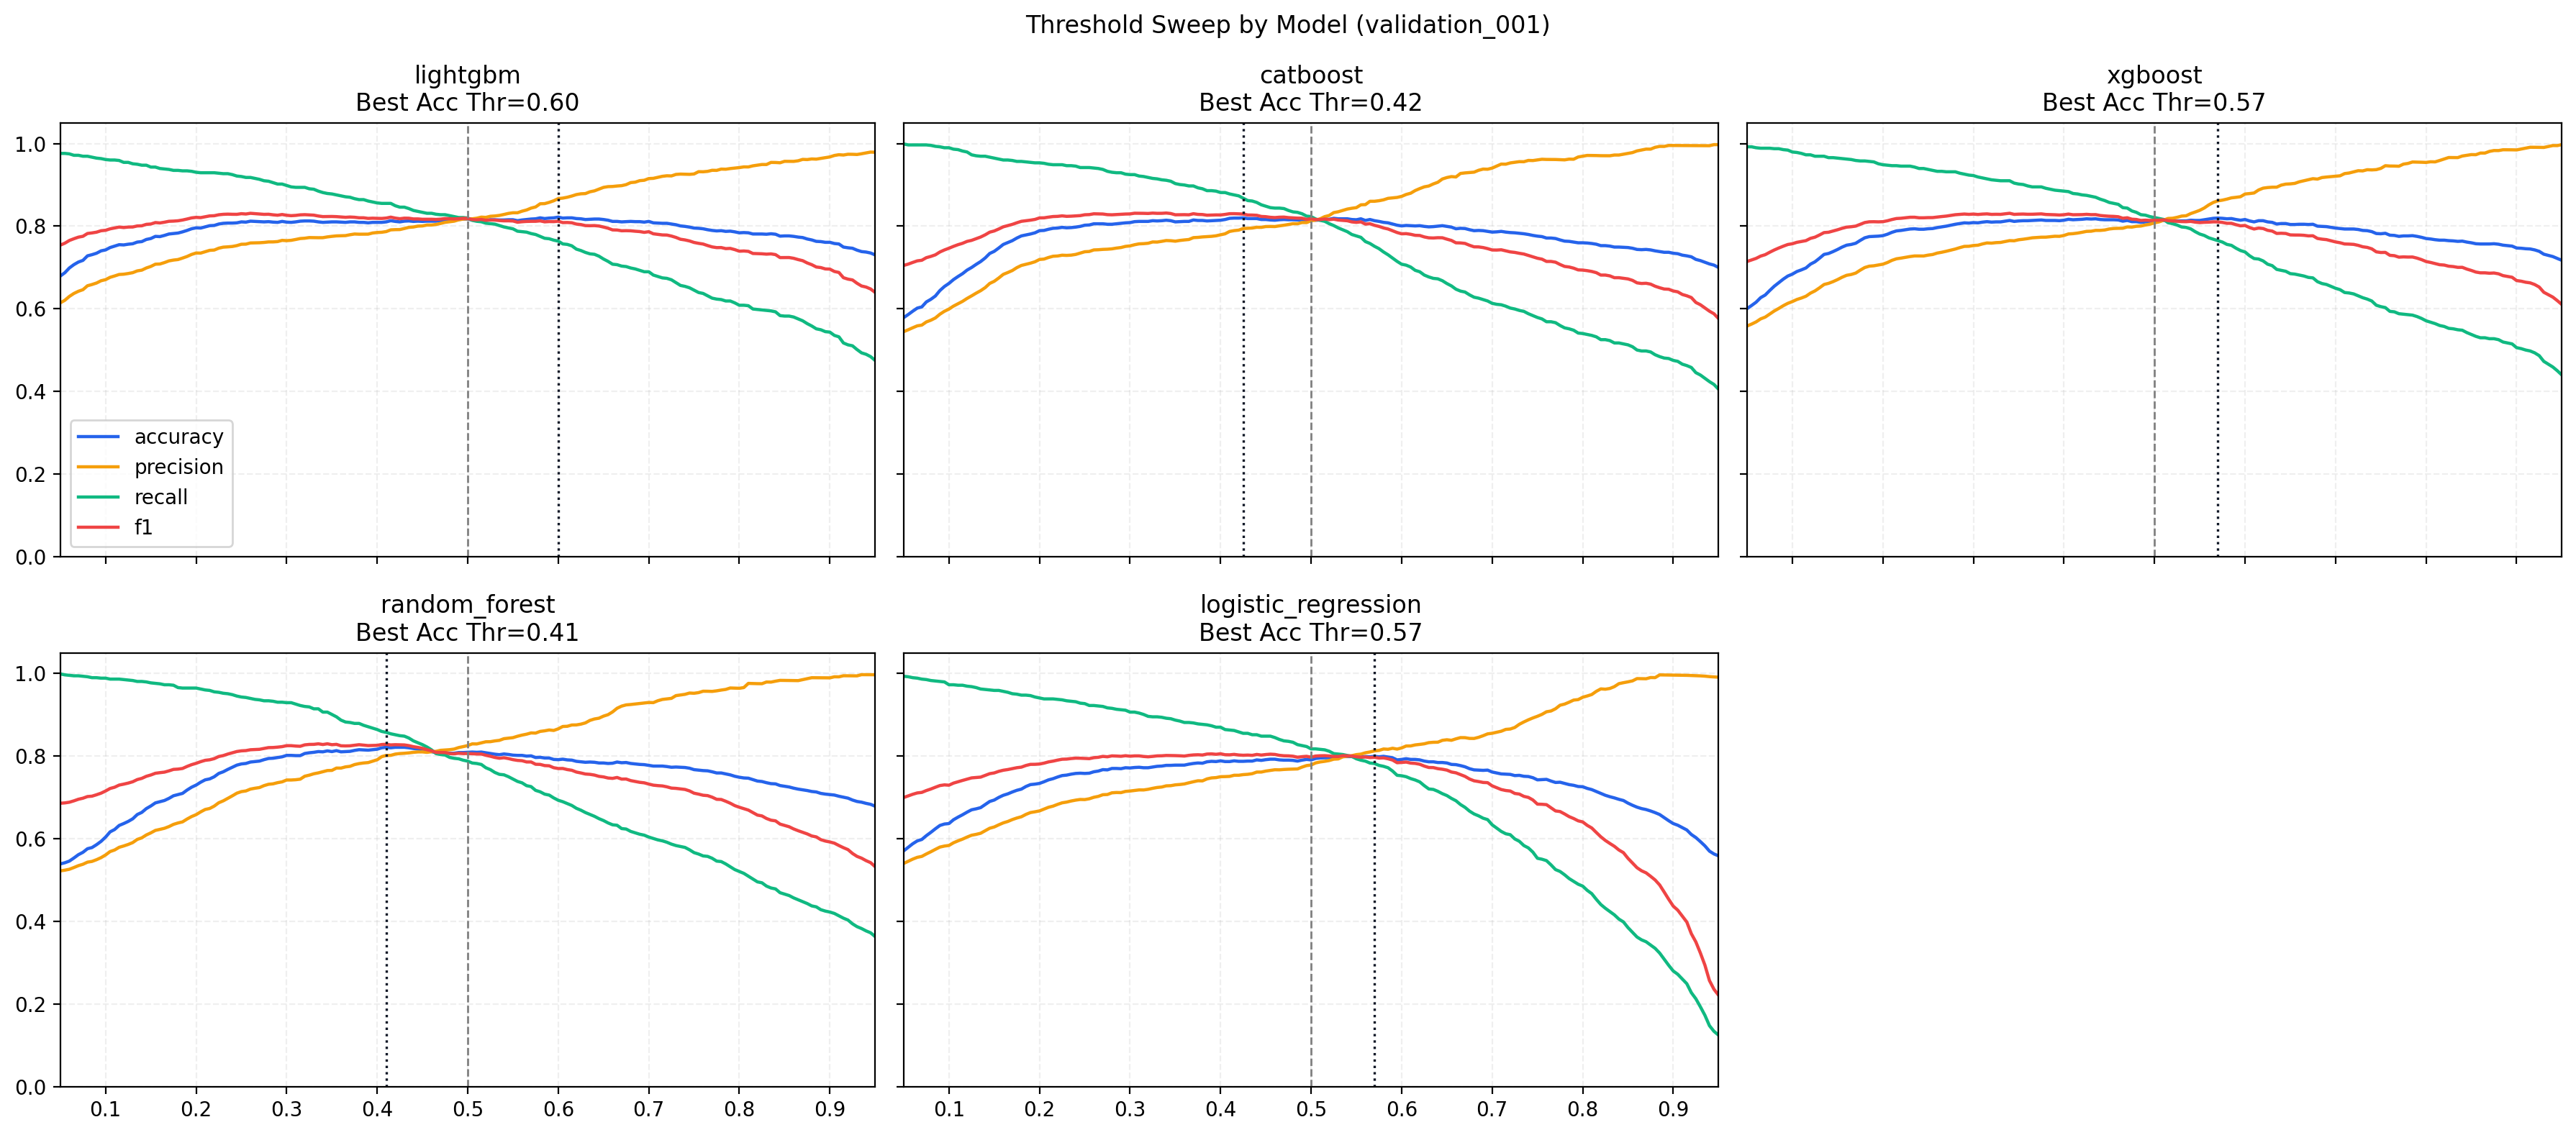
\includegraphics[width=\linewidth]{figures/validation_threshold_sweep_by_model.png}
\caption{Model-specific threshold sweeps for the local validation split. Each panel shows how accuracy, precision, recall, and F1 change with the classification threshold, while the dotted line marks the accuracy-maximizing threshold for that model. LightGBM and XGBoost achieve their best plotted accuracy at slightly higher thresholds, whereas CatBoost and Random Forest peak at lower thresholds, indicating that the default threshold of 0.5 is reasonable but not always optimal for every classifier.}
\label{fig:threshold_by_model}
\end{figure}

\begin{figure}[t]
\centering
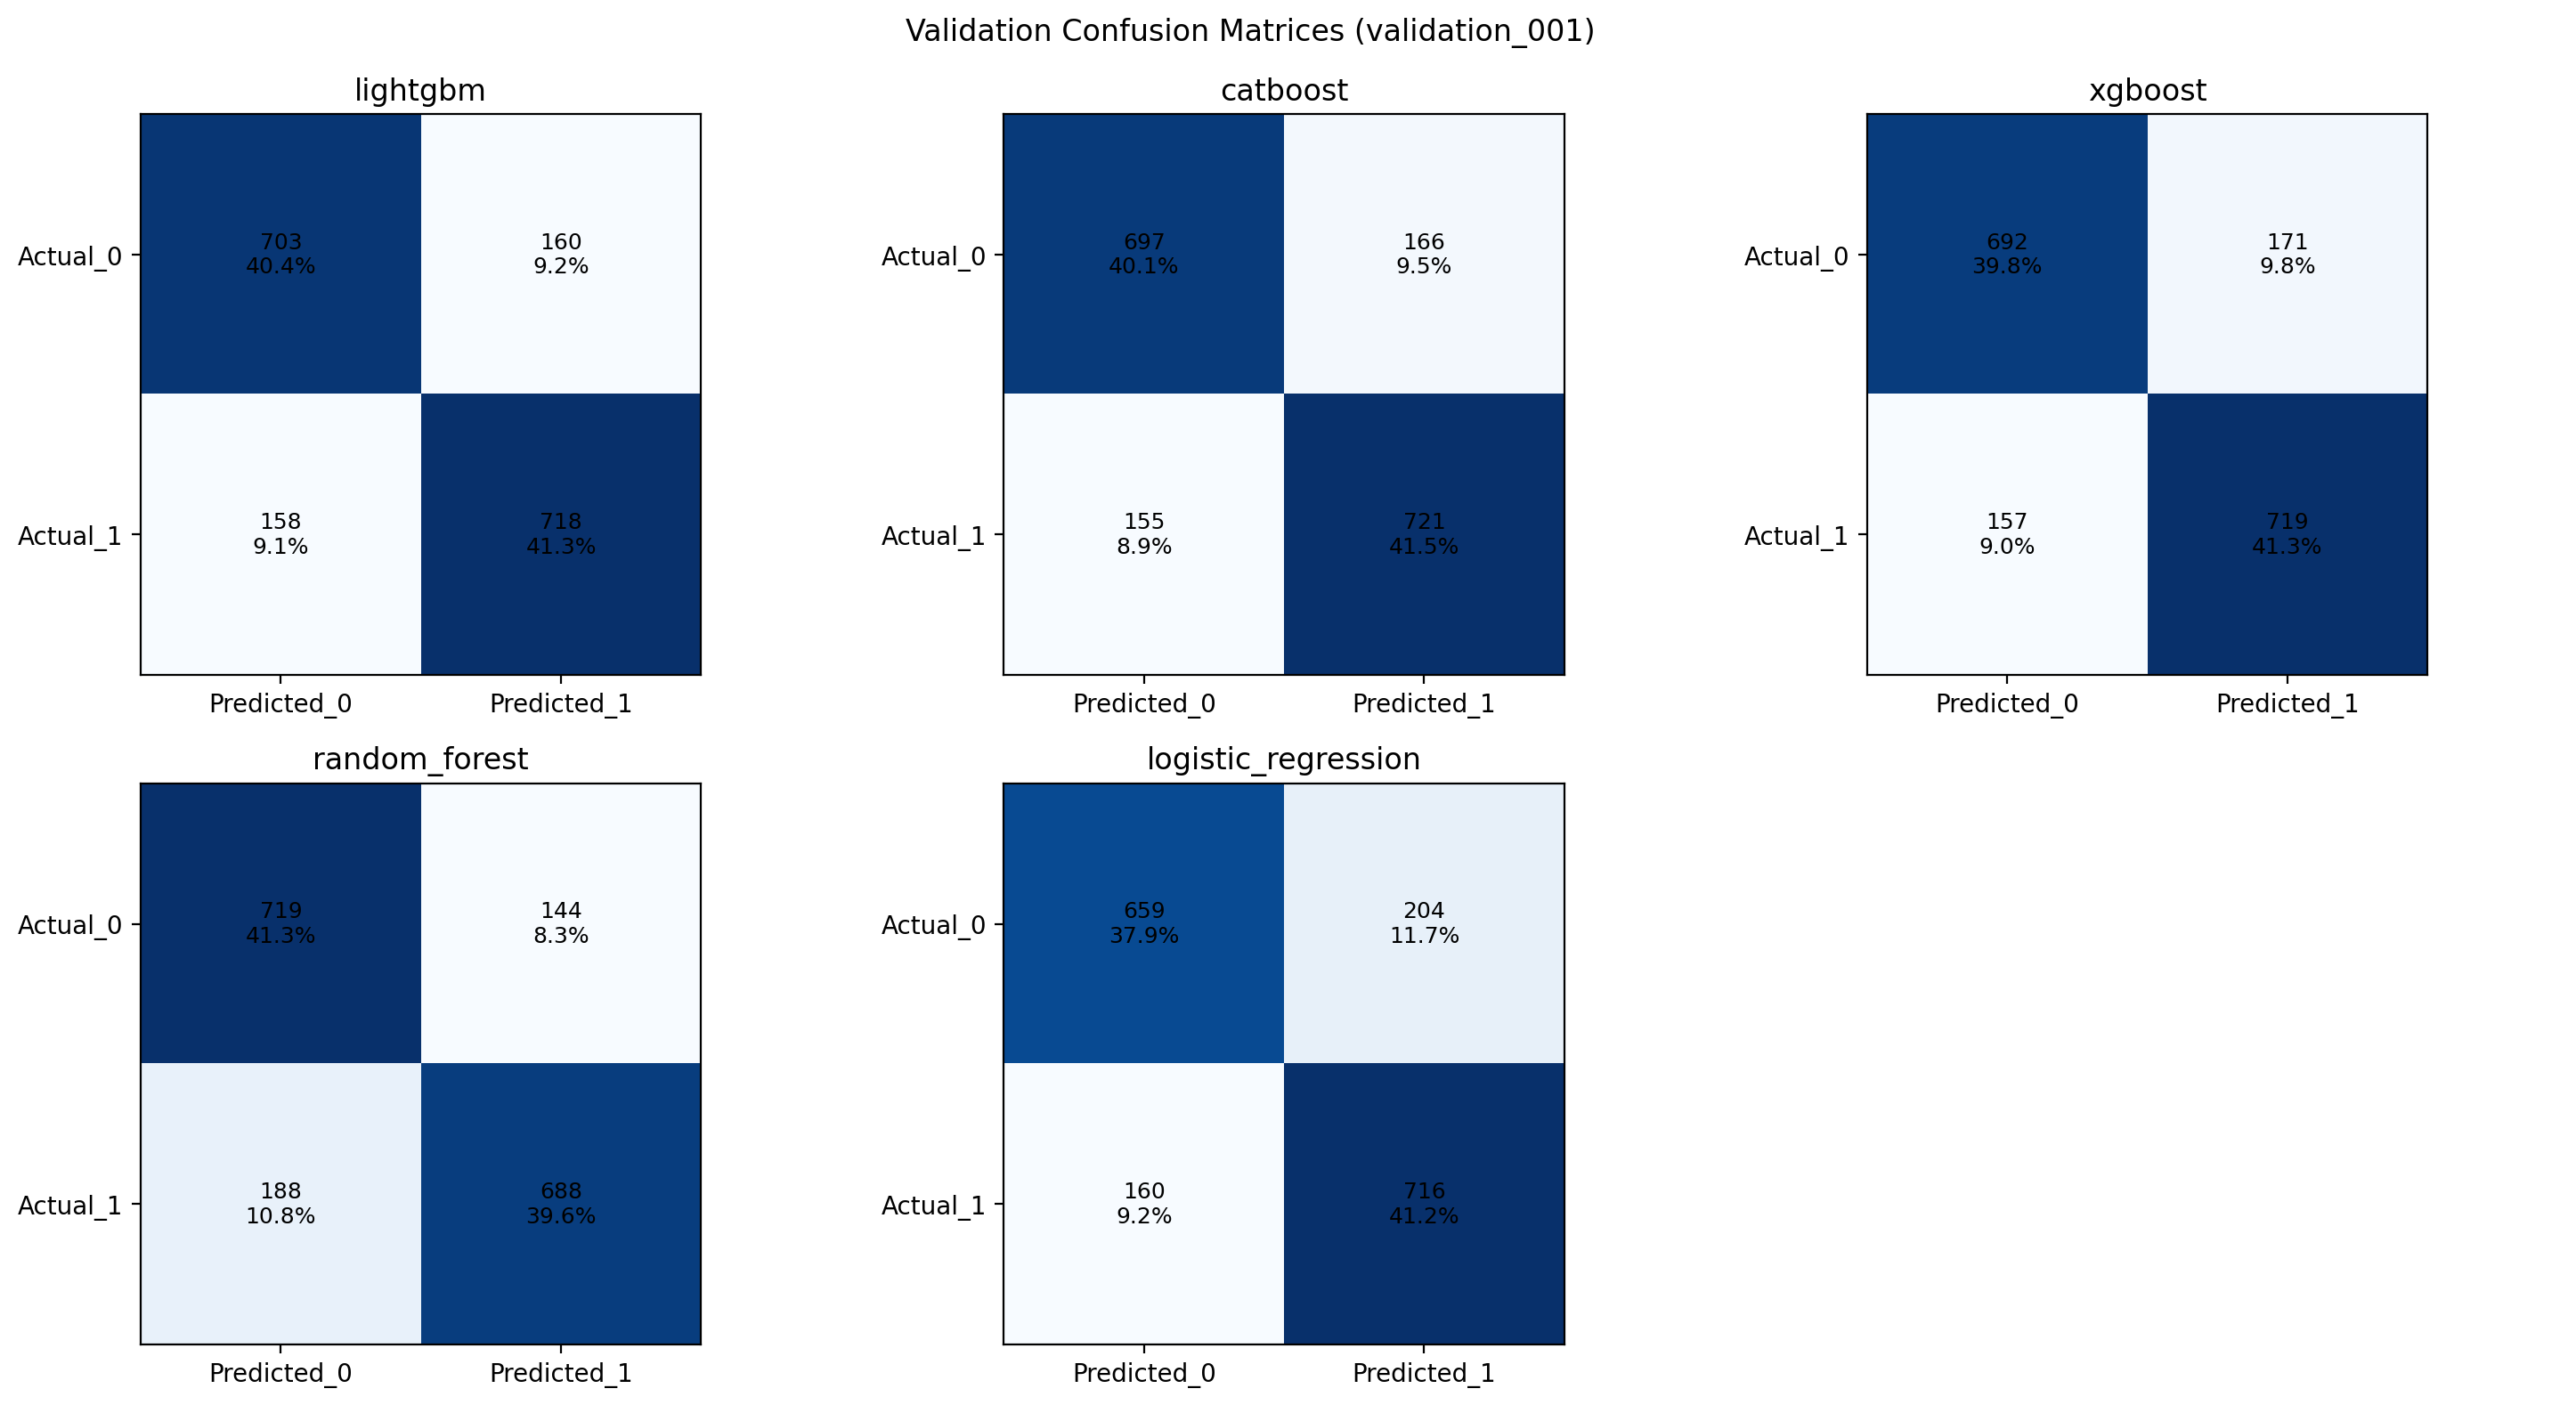
\includegraphics[width=\linewidth]{figures/validation_confusion_matrices.png}
\caption{Confusion matrices for the local validation split. LightGBM, CatBoost, and XGBoost show the most balanced error profiles, with strong true-negative and true-positive counts and comparatively limited off-diagonal errors. Random Forest is slightly more conservative and misses more positive cases, while Logistic Regression produces the largest false-positive count, which is consistent with its lower overall precision and accuracy.}
\label{fig:confusion_matrices}
\end{figure}

\begin{figure}[t]
\centering
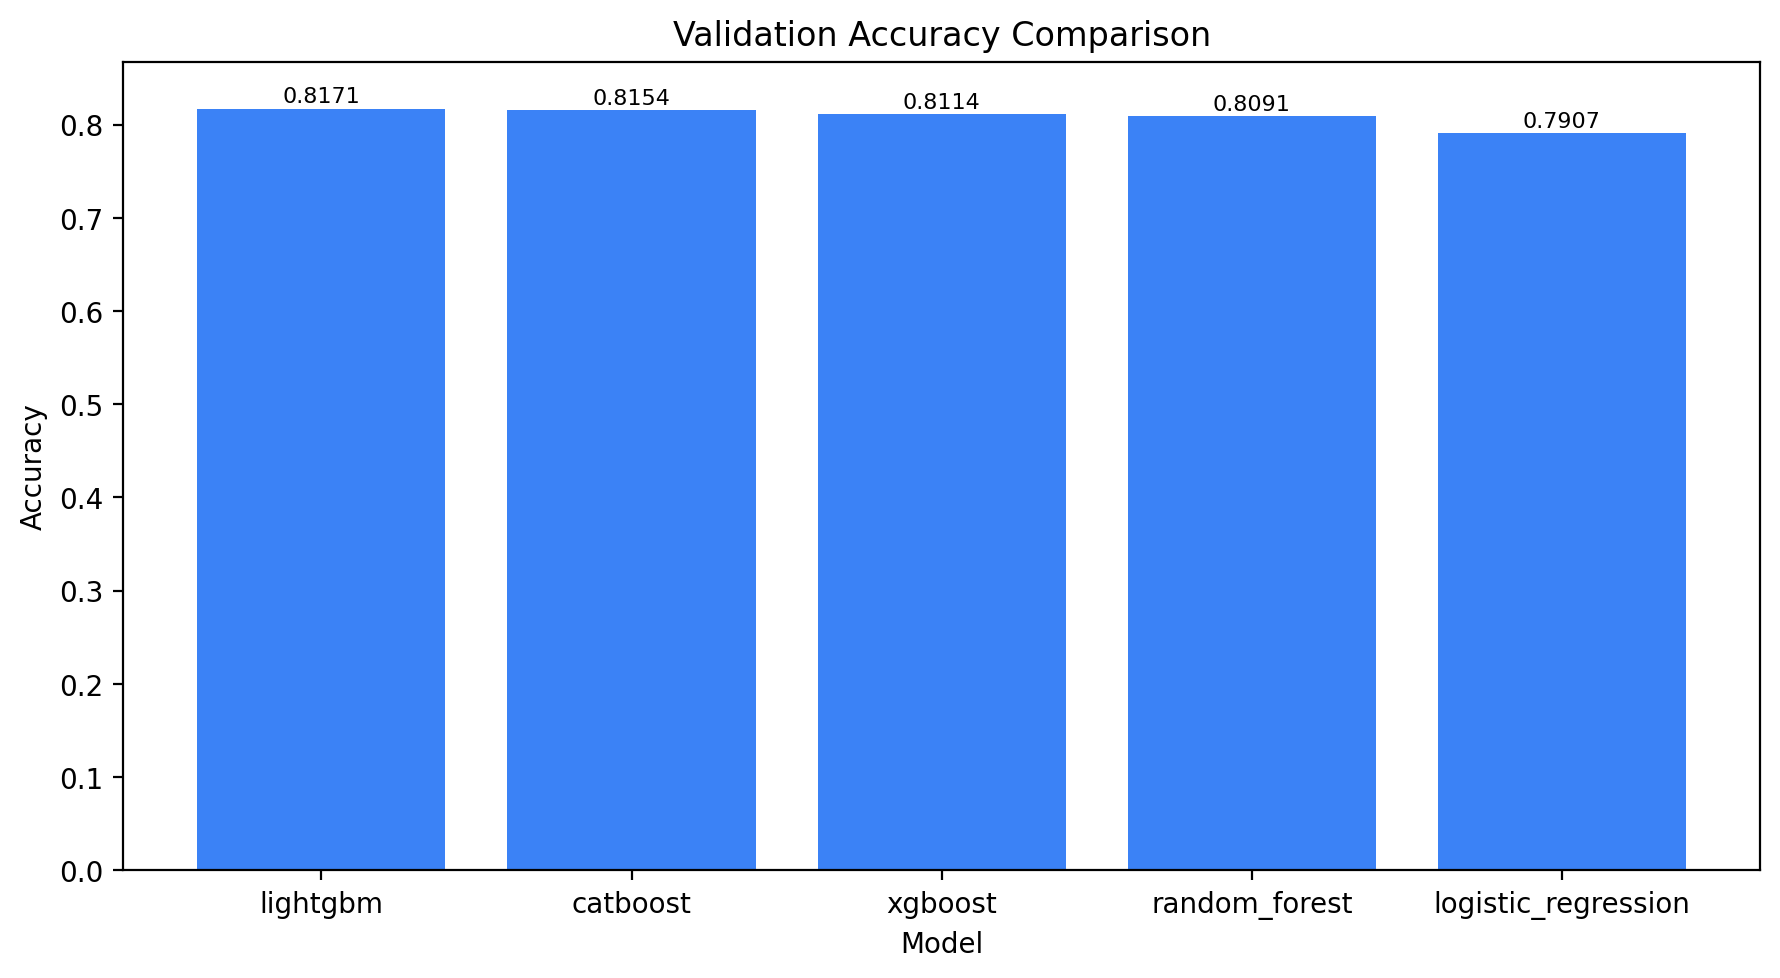
\includegraphics[width=\linewidth]{figures/validation_accuracy_comparison.png}
\caption{Accuracy ranking across the five evaluated models on the local validation split. LightGBM achieves the highest validation accuracy (0.8171), followed closely by CatBoost (0.8154) and XGBoost (0.8114), while Random Forest remains competitive and Logistic Regression ranks last. The small gap among the top tree-based models suggests that the leading methods perform similarly under the same preprocessing and evaluation protocol.}
\label{fig:accuracy_ranking}
\end{figure}

\begin{figure}[t]
\centering
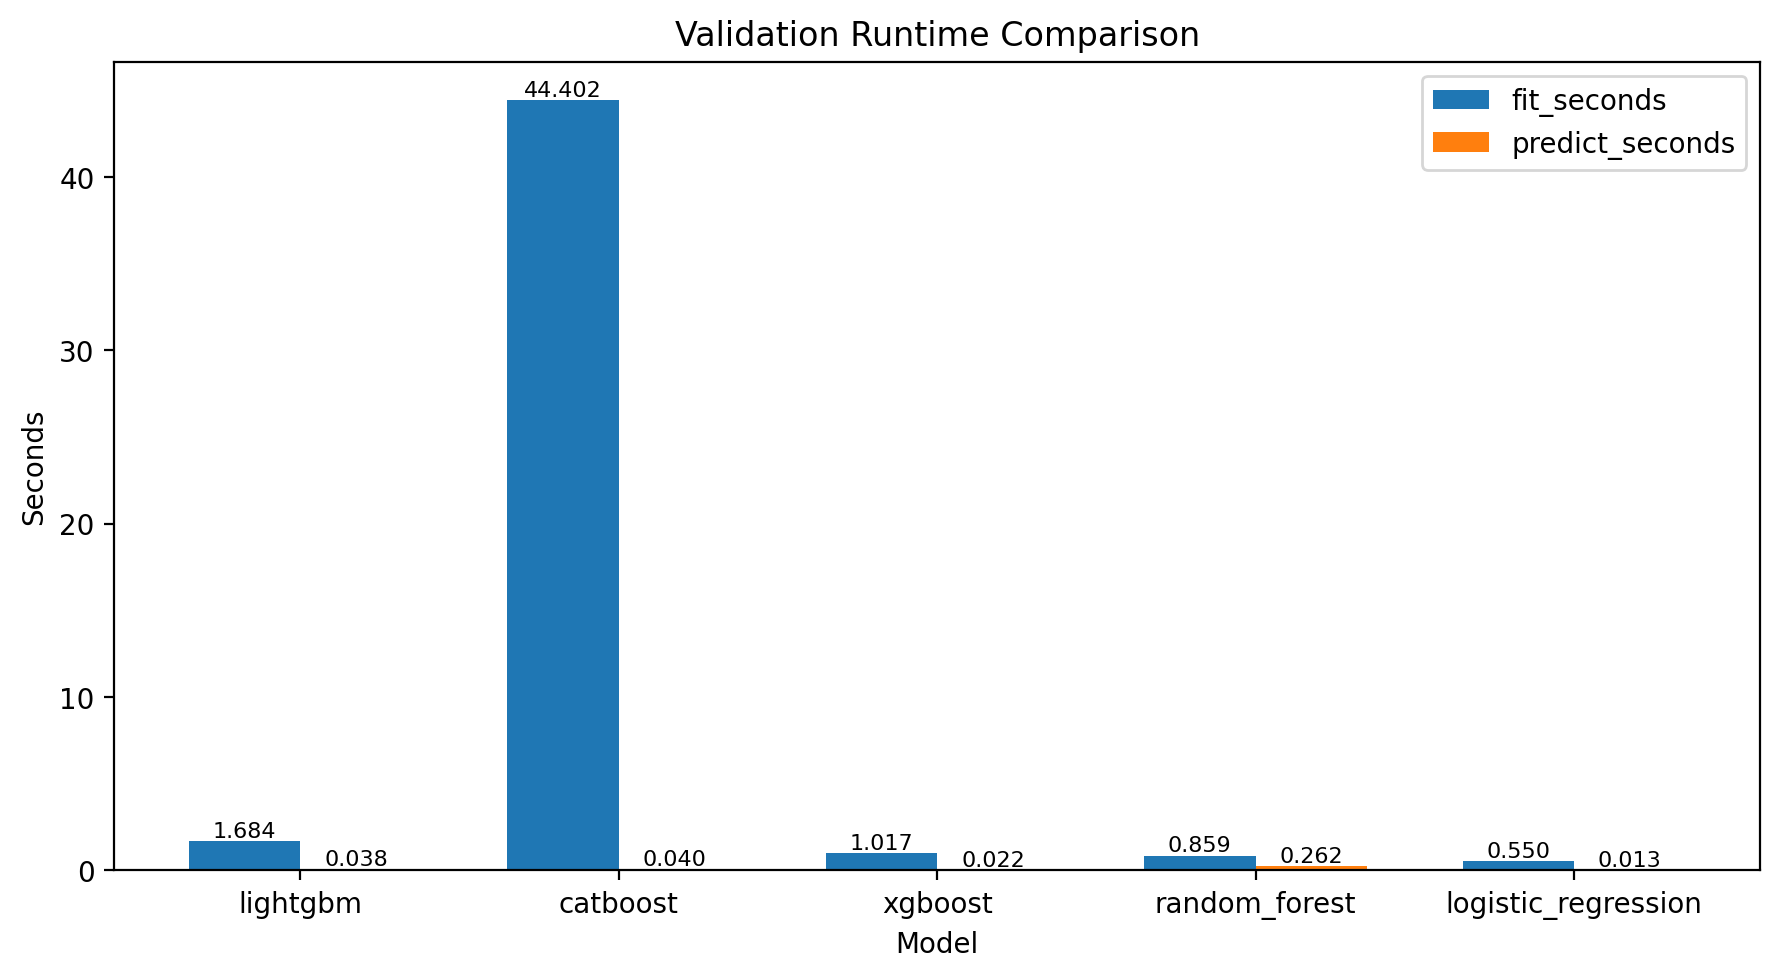
\includegraphics[width=\linewidth]{figures/validation_runtime_comparison.png}
\caption{Training and inference runtime comparison across models. Logistic Regression, XGBoost, and LightGBM train quickly, whereas CatBoost has by far the largest training cost at about 44.4 seconds. Prediction time remains low for all models, although Random Forest shows relatively slower inference, so the main efficiency difference in this experiment comes from training rather than deployment latency.}
\label{fig:runtime_comparison}
\end{figure}

\begin{figure}[t]
\centering
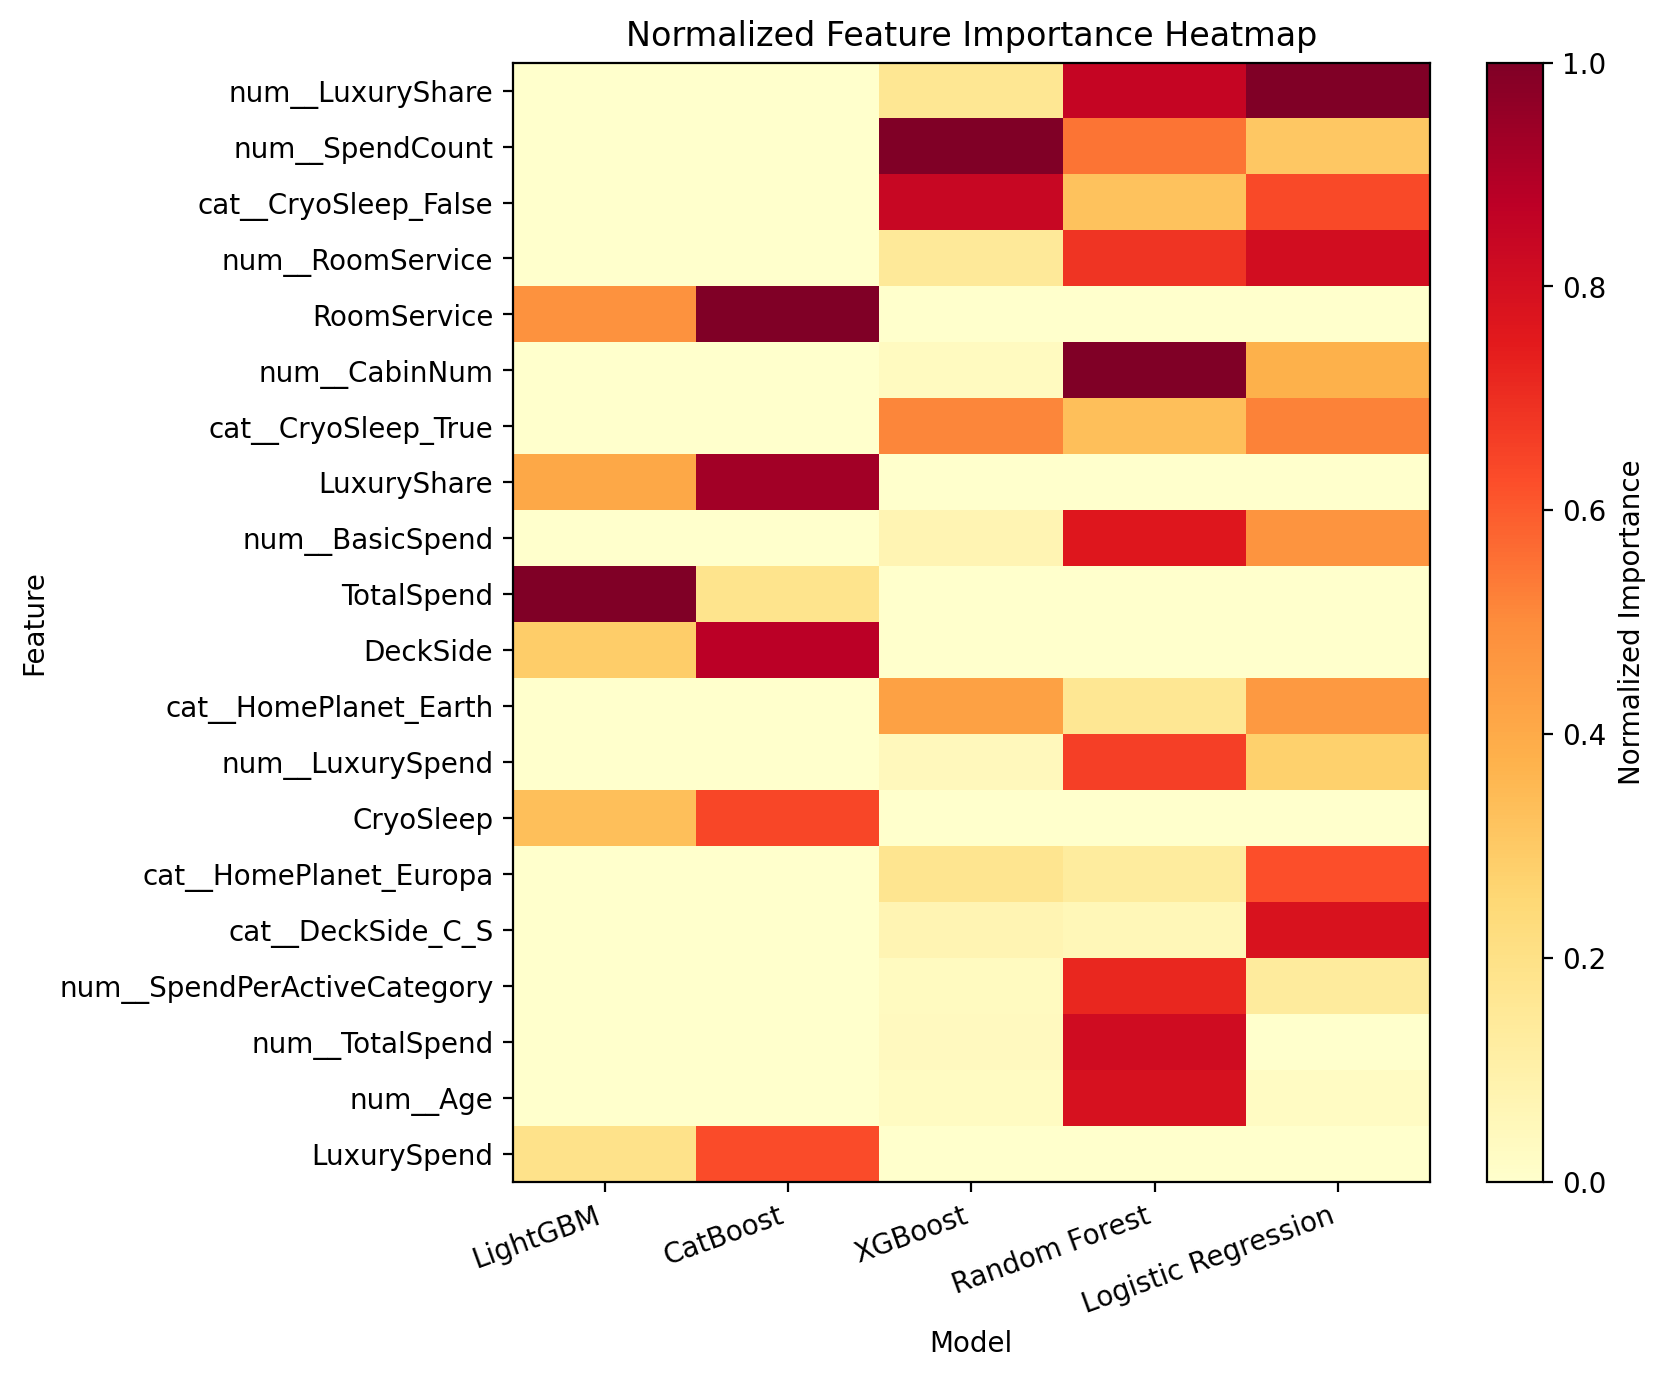
\includegraphics[width=\linewidth]{figures/validation_feature_importance_heatmap.png}
\caption{Normalized feature-importance heatmap across all models. Spending-related variables, CryoSleep indicators, and cabin or location features appear repeatedly among the most influential predictors, but the relative emphasis differs by algorithm. Because all values are normalized before plotting, this figure should be interpreted as a comparison of importance patterns across models rather than a comparison of absolute importance magnitudes.}
\label{fig:importance_heatmap}
\end{figure}

\begin{thebibliography}{30}
\bibitem{kaggle_spaceship_titanic} Kaggle, ``Spaceship Titanic,'' 2022. [Online]. Available: https://www.kaggle.com/competitions/spaceship-titanic
\bibitem{borisov2024tabularsurvey} V. Borisov et al., ``Deep neural networks and tabular data: A survey,'' IEEE TNNLS, vol. 35, no. 6, pp. 7499--7519, 2024.
\bibitem{grinsztajn2022trees} L. Grinsztajn, E. Oyallon, and G. Varoquaux, ``Why do tree-based models still outperform deep learning on typical tabular data?'' NeurIPS, 2022.
\bibitem{mcelfresh2023nnsvstrees} D. C. McElfresh et al., ``When do neural nets outperform boosted trees on tabular data?'' NeurIPS, 2023.
\bibitem{grinsztajn2024betterdefault} D. Holzmuller, L. Grinsztajn, and I. Steinwart, ``Better by default: Strong pre-tuned MLPs and boosted trees on tabular data,'' NeurIPS, 2024.
\bibitem{tschalzev2024datacentric} A. Tschalzev et al., ``A data-centric perspective on evaluating machine learning models for tabular data,'' NeurIPS, 2024.
\bibitem{kapoor2023leakage} S. Kapoor and A. Narayanan, ``Leakage and the reproducibility crisis in machine-learning-based science,'' Patterns, vol. 4, no. 9, 2023.
\bibitem{kapoor2024reforms} S. Kapoor et al., ``REFORMS: Consensus-based recommendations for machine-learning-based science,'' Science Advances, vol. 10, no. 18, 2024.
\bibitem{chicco2022tips} D. Chicco, L. Oneto, and E. Tavazzi, ``Eleven quick tips for data cleaning and feature engineering,'' PLOS Computational Biology, vol. 18, no. 12, 2022.
\bibitem{josse2024missingconsistency} J. Josse et al., ``On the consistency of supervised learning with missing values,'' Statistical Papers, vol. 65, no. 9, pp. 5447--5479, 2024.
\bibitem{zhou2024missingreview} Y. Zhou, S. Aryal, and M. R. Bouadjenek, ``Review for handling missing data with special missing mechanism,'' arXiv preprint arXiv:2404.04905, 2024.
\bibitem{jarrett2022hyperimpute} D. Jarrett et al., ``Hyperimpute: Generalized iterative imputation with automatic model selection,'' arXiv:2206.07769, 2022.
\bibitem{matteucci2023encoders} F. Matteucci, V. Arzamasov, and K. Bohm, ``A benchmark of categorical encoders for binary classification,'' NeurIPS, 2023.
\bibitem{avanzi2023highcardinality} B. Avanzi, G. Taylor, M. Wang, and B. Wong, ``Machine learning with high-cardinality categorical features in actuarial applications,'' arXiv:2301.12710, 2023.
\bibitem{scikit_learn} F. Pedregosa et al., ``Scikit-learn: Machine learning in Python,'' JMLR, vol. 12, pp. 2825--2830, 2011.
\bibitem{rudin2019interpretable} C. Rudin, ``Stop explaining black box machine learning models for high stakes decisions and use interpretable models instead,'' Nature Machine Intelligence, vol. 1, no. 5, pp. 206--215, 2019.
\bibitem{dervovic2024logistic} D. Dervovic et al., ``Are logistic models really interpretable?'' IJCAI, 2024.
\bibitem{random_forest} L. Breiman, ``Random forests,'' Machine Learning, vol. 45, no. 1, pp. 5--32, Oct. 2001, doi: 10.1023/A:1010933404324.
\bibitem{rothacher2024rfvarselect} G. Louppe, L. Wehenkel, A. Sutera, and P. Geurts, ``Understanding variable importances in forests of randomized trees,'' in Proc. 26th Int. Conf. Neural Information Processing Systems (NIPS), 2013, pp. 431--439.
\bibitem{xgboost} T. Chen and C. Guestrin, ``XGBoost: A scalable tree boosting system,'' KDD, pp. 785--794, 2016.
\bibitem{lightgbm} G. Ke et al., ``LightGBM: A highly efficient gradient boosting decision tree,'' NeurIPS, vol. 30, 2017.
\bibitem{salinas2024tabrepo} D. Salinas and N. Erickson, ``TabRepo: A large scale repository of tabular model evaluations and its AutoML applications,'' ICML AutoML, 2024.
\bibitem{catboost} L. Prokhorenkova, G. Gusev, A. Vorobev, A. V. Dorogush, and A. Gulin, ``CatBoost: Unbiased boosting with categorical features,'' in Proc. 32nd Int. Conf. Neural Information Processing Systems (NeurIPS), 2018, pp. 6639--6649.
\bibitem{silva2023calibration} T. Silva Filho et al., ``Classifier calibration: A survey on how to assess and improve predicted class probabilities,'' Machine Learning, vol. 112, no. 9, 2023.
\bibitem{lee2023tcal} D. Lee, X. Huang, H. Hassani, and E. Dobriban, ``T-cal: An optimal test for the calibration of predictive models,'' JMLR, vol. 24, no. 335, 2023.
\bibitem{leevy2023threshold} J. L. Leevy et al., ``Threshold optimization and random undersampling for imbalanced credit card data,'' Journal of Big Data, vol. 10, no. 1, 2023.
\bibitem{lundberg2017shap} S. M. Lundberg and S.-I. Lee, ``A unified approach to interpreting model predictions,'' NeurIPS, vol. 30, 2017.
\bibitem{strobl2007bias} C. Strobl, A.-L. Boulesteix, A. Zeileis, and T. Hothorn, ``Bias in random forest variable importance measures: Illustrations, sources and a solution,'' BMC Bioinformatics, vol. 8, no. 25, 2007.
\bibitem{somvanshi2024deeptabular} S. Somvanshi et al., ``A survey on deep tabular learning,'' arXiv:2410.12034, 2024.
\end{thebibliography}

\end{document}
